%the entire chapter is edited
% entered all footnotes
\باب{قواعد و ضوابط}\شناخت{باب_قواعد_و_ضوابط}
%======================

\حصہ{ہلبرٹ فضا}
گزشتہ دو ابواب میں سادہ ہارمونی نظاموں کے چند دلچسپ خواص ہماری نظروں سے گزرے۔ان میں سے چند ایک مخصوص مخفیہ کے  "ناگہاں" خدوخال تھے ( مثلاً ہارمونی مرتعش میں توانائی کی سطح میں جفت فاصلے) جبکہ باقی (مثلاً عدم یقینیت کا اصول اور ساکن حالات کی عمودیت) زیادہ عمومی معلوم ہوتے ہیں، جنہیں ایک ہی مرتبہ ثابت کرنا مفید  ہوگا۔ اس کو مد نظر رکھتے ہوئے اس باب میں نظریہ کو زیادہ مضبوط روپ میں پیش کیا جائے گا۔ یہاں کوئی نئی بات نہیں کی جائے گی بلکہ مخصوص صورتوں میں دیکھے گئے خواص سے معقول نتائج اخذ کیے جائیں گے۔
	
کوانٹائی نظریہ کا دارومدار\ترچھا{ تفاعل موج} اور \ترچھا{عاملین} کے تصور پر مبنی ہے۔ نظام کے حال کو تفاعل موج ظاہر کرتا ہے جبکہ قابل مشاہدہ کو عاملین ظاہر کرتے ہیں۔ تفاعل موج،  ریاضیاتی طور پر،  تصوراتی \اصطلاح{سمتیات}\فرہنگ{سمتیات}\حاشیہب{vectors}\فرہنگ{vectors} کی تعریفی شرائط پر پورے اترتے ہیں؛  جبکہ عاملین ان پر \اصطلاح{خطی تبادلہ}\فرہنگ{خطی تبادلہ}\حاشیہب{linear transformations}\فرہنگ{transformations!linear} کا عمل کرتے ہیں۔ یوں کوانٹم میکانیات کی قدرتی زبان \اصطلاح{خطی الجبرا}\فرہنگ{خطی الجبرا}\حاشیہب{linear algebra}\فرہنگ{linear algebra}\حاشیہد{آگے بڑھنے سے پہلے بہتر ہو گا کہ آپ ضمیمہ پڑھ کر خطی الجبرا سیکھیں۔} ہے۔
	
 مجھے خدشہ ہے کہ یہاں مستعمل خطی الجبرا سے آپ واقف نہیں ہوں گے۔ سمتیہ\عددی{|\alpha\rangle} کو \عددی{N} بُعدی فضا میں کسی مخصوص معیاری عمودی اساس کے لحاظ سے \عددی{N} عدد اجزاء 
\عددی{\{a_n\}} سے ظاہر کرنا سادہ ترین ثابت ہوتا ہے۔
	\begin{align}
		|\alpha \rangle \rightarrow \mat{a} = \begin{pmatrix} 
			a_{1}\\
			a_{2}\\
			\vdots\\
			a_{N}
		 \end{pmatrix}
	\end{align}
 دو سمتیات کا \اصطلاح{اندرونی ضرب }\فرہنگ{اندرونی ضرب}\حاشیہب{inner product}\فرہنگ{inner product}
 \عددی{\langle\alpha|\beta\rangle} (تین ابعادی نقطہ ضرب کو وسعت دیتے ہوئے) درج ذیل مخلوط عدد ہوگا۔
\begin{align}\label{مساوات_قواعد_اندرونی_ضرب}
	\langle \alpha | \beta\rangle =a_1^{\ast}b_1 + a_2^{\ast}b_2 + \dotsb +a_N^{\ast}b_N
\end{align}
خطی تبادلہ، \عددی{ T}، کو (کسی مخصوص اساس کے لحاظ سے ) \اصطلاح{قوالب}\فرہنگ{قوالب}\حاشیہب{matrices}\فرہنگ{matrices} سے ظاہر کیا جاتا ہے، جو قالبی ضرب کے سادہ قواعد کے تحت سمتیات پر عمل کرتے ( ہوئے نئے سمتیات پیدا کرتے) ہیں:
\begin{align}
	|\beta\rangle = T|\alpha \rangle \rightarrow \mat{b} = \mat{T}\mat{a} = \begin{pmatrix}
		t_{11} & t_{12} & \hdots & t_{1N} \\ 
		t_{21} & t_{22} & \hdots & t_{2N} \\
		\vdots & \vdots & & \vdots \\
		t_{N1} & t_{N2} & \hdots & t_{NN} 
	\end{pmatrix}
\begin{pmatrix}
	a_{1}\\
	a_{2}\\
	\vdots\\
	a_{N}
\end{pmatrix}
\end{align}
کوانٹم میکانیات میں پائے جانے والے "سمتیات" درحقیقت ( زیادہ تر) تفاعلات ہوتے ہیں جو لامتناہی بُعدی فضا میں بستے ہیں۔ انہیں \عددی{N} اجزائی قالبی علامت سے ظاہر کرنا زیادہ ٹھیک نہیں ہوگا اور متناہی ابعاد  میں  سمجھ آنے والی ٹھیک وضاحتیں ، لامتناہی ابعاد  میں پریشان کن ثابت ہو سکتی  ہیں۔ ( اس کی بنیادی وجہ یہ ہے کہ  مساوات \حوالہ{مساوات_قواعد_اندرونی_ضرب} کا متناہی مجموعہ ہر صورت موجود ہوتا ہے،البتہ،  لا متناہی مجموعہ یا تکمل،  عدم مرکوزیت کا شکار ہو سکتا ہے، اور ایسی صورت میں اندرونی ضرب غیر موجود ہوگی لہٰذا اندرونی ضرب پر مبنی کوئی بھی دلیل مشکوک ہوگی۔) یوں اگرچہ خطی الجبرا کی اصطلاحات اور علامتیت سے آپ واقف ہوں گے، بہرحال ہوشیار رہنا بہتر ہو گا۔

متغیر \عددی{x} کے تمام تفاعلات مل کر سمتی فضا قائم کرتے ہیں، جو ہمارے مقصد کے لئے  ضرورت سے زیادہ بڑی فضا ہے۔ کسی بھی ممکنہ طبیعی حال کو ظاہر کرنے کے لیے لازم ہے کہ تفاعل موج
\عددی{\Psi} \ترچھا{معمول شدہ} ہو:
\begin{align*}
\int \abs{\Psi}^2 \dif x = 1
\end{align*}
کسی مخصوص وقفہ\حاشیہد{ہمارے لئے حدود  (\عددی{a} اور \عددی{b}) تقریباً ہر مرتبہ \عددی{\pm\infty} ہوں گی، تاہم یہاں چیزوں کو زیادہ عمومی رکھنا بہتر ہو گا۔} پر تمام \اصطلاح{ مربع متکامل تفاعلات}\فرہنگ{مربع متکامل تفاعلات}\حاشیہب{square-integrable functions}\فرہنگ{square-integrable functions}
\begin{align}
 \text{\RL{ہو}}\quad \int_{a}^b |f(x)|^2 \dif x < \infty \quad \text{جہاں}\quad f(x) 
\end{align}
مل کر( اس سے بہت چھوٹی) سمتی فضا قائم کرتے ہیں ( سوال \حوالہ{سوال_قواعد_مربع_قابل_تکمل}-ا دیکھیں)۔ ریاضی دان اسے \عددی{L_2 (a,b)} جبکہ ماہر طبیعیات اسے \اصطلاح{ہلبرٹ فضا }\فرہنگ{ہلبرٹ فضا}\حاشیہب{Hilbert space}\فرہنگ{Hilbert space}کہتے\حاشیہد{تکنیکی طور پر، ہلبرٹ فضا سے مراد \اصطلاح{مکمل اندرونی ضرب فضا} ہے، اور مربع متکامل تفاعلات کا ذخیرہ ہلبرٹ فضا کی فقط ایک مثال ہے؛ درحقیقت، ہر متناہی ابعادی سمتی فضا ایک بے وقعت  ہلبرٹ فضا ہو گی۔چونکہ  \عددی{L_2}  کوانٹم میکانیات کا اکھاڑا ہے لہٰذا ماہر طبیعیات اسی کو" ہلبرٹ فضا" کہتے ہیں۔ویسے یہاں لفظ \اصطلاح{مکمل} سے مراد یہ ہے کہ ہلبرٹ فضا  کے کسی بھی تفاعل کی کوشی ترتیب جس تفاعل پر مرکوز ہو، وہ اسی فضا میں پایا جائے۔  اس میں کوئی "سوراخ" نہیں پایا جاتا، جیسا کہ تمام حقیقی اعداد کے سلسلہ میں کوئی سوراخ نہیں پایا  جاتا (اس کے برعکس،مثلاً، تمام کثیر رکنیوں کی فضا میں اور تمام ناطق اعداد کے سلسلہ میں یقیناً  سوراخ پائے جاتے ہیں)۔فضا کی مکملیت کا   تفاعلات کے سلسلہ کی مکملیت کے ساتھ  (ایک ہی لفظ استعمال کیے جانے کے باوجود) کوئی تعلق نہیں۔ تفاعلات کی مکملیت سے مراد یہ ہے کہ کسی بھی تفاعل کو ان تفاعلات کے خطی جوڑ کی صورت میں  لکھا جا سکتا ہے۔ } ہیں۔ یوں کوانٹم میکانیات میں
\begin{align}\label{مساوات_قواعد_ہلبرٹ_بستے}
	\text{\RL{\موٹا{تفاعلات موج ہلبرٹ فضا میں بستے ہیں۔}}}
\end{align}
 \موٹا{دو تفاعلات کی  اندرونی ضرب} کی تعریف درج ذیل  ہے جہاں \عددی{f(x)} اور \عددی{g(x)} تفاعلات ہیں۔
\begin{align}\label{مساوات_قواعد_دو_تفاعلات_کا_اندرونی_ضرب}
	\langle f | g \rangle \equiv \int_{a}^b f(x)^{\ast} g(x) \dif x
\end{align}
اگر \عددی{ f} اور \عددی{g} دونوں   مربع متکامل  ہوں ( یعنی دونوں ہلبرٹ فضا میں پائے جاتے ہوں)،    تب ہم ضمانت کے ساتھ کہہ سکتے ہیں کہ ان کی اندرونی ضرب موجود ہوگی
( مساوات \حوالہ{مساوات_قواعد_دو_تفاعلات_کا_اندرونی_ضرب} کا تکمل ایک متناہی عدد\حاشیہد{باب \حوالہ{باب_غیر_تابع_وقت_شروڈنگر_مساوات} میں بعض اوقات ہمیں مجبوراً  معمول پر نہ لانے کے قابل   تفاعلات کے ساتھ  کام کرنا پڑا ۔ایسے تفاعلات ہلبرٹ فضا سے باہر بستے ہیں، اور جیسا آپ جلد دیکھیں گے،  انہیں استعمال کرتے ہوئے ہمیں احتیاط کرنی ہو گی۔ ابھی  کے لئے میں فرض  کرتا ہوں کہ جن تفاعلات سے ہمیں واسطہ ہے وہ ہلبرٹ فضا میں بستے ہیں۔ } پر مرکوز ہوگا)۔   ایسا \اصطلاح{شوارز عدم مساوات}\فرہنگ{شوارز عدم مساوات}\حاشیہب{Schwarz inequality}\فرہنگ{Schwarz inequality} کے  درج ذیل تکملی روپ\حاشیہد{متناہی ابعادی سمتی فضا میں شوارز عدم مساوات \عددی{\abs{\langle\alpha|\beta\rangle}^2\le \langle\alpha|\alpha\rangle\langle\beta|\beta\rangle} کو ثابت کرنا آسان ہے (صفحہ \حوالہصفحہ{ضمیمہ_اندرونی_ضرب_شوارز_عدم_مساوات_ثبوت} پر سوال \حوالہ{ضمیمہ_اندرونی_ضرب_شوارز_عدم_مساوات_ثبوت} دیکھیں)۔ تاہم یہ ثبوت فرض کرتا ہے کہ جن تفاعلات سے ہمیں واسطہ ہے وہ ہلبرٹ فضا میں پائے جاتے ہیں، جبکہ ہم یہاں اسی حقیقت کو ثابت کرنا چاہتے ہیں۔} کے پیش نظر ہوگا۔
\begin{align}\label{مساوات_قواعد_شوارٹز_عدم}
	\abs{\int_{a}^b f(x)^{\ast} g(x) \dif x} \leq \sqrt{\int_{a}^b \abs{f(x)}^2 \dif x \int_{a}^b \abs{g(x)}^2 \dif x}
\end{align}
آپ تصدیق کر سکتے ہیں کہ مساوات \حوالہ{مساوات_قواعد_دو_تفاعلات_کا_اندرونی_ضرب} اندرونی ضرب کی تمام  شرائط پر پوری  اترتی ہے (سوال \حوالہ{سوال_قواعد_مربع_قابل_تکمل}-ب)۔ بالخصوص درج ذیل مساوات میں  ہم دیکھ سکتے ہیں ۔
\begin{align}\label{مساوات_قواعد_مخلوط_جوڑی_دار_الٹ_ترتیب}
	\langle g | f \rangle = \langle f | g \rangle^{\ast}
\end{align} 
مزید  \عددی{f(x)}  کی اپنے ہی ساتھ اندرونی ضرب
\begin{align}\label{مساوات_قواعد_اپنے_ساتھ_اندرونی_ضرب}
	\langle f | f \rangle = \int_{a}^b \abs{f(x)}^2 \dif x
\end{align}
\ترچھا{حقیقی}  اور غیر منفی ہوگی؛  یہ صرف اس صورت\حاشیہد{ایسے تفاعل کے لئے کیا  کہا جا سکتا ہے  جو  چند مخصوص تنہا نقاط  کے علاوہ ہر مقام پر صفر ہوں؟  اگرچہ تفاعل  معدوم نہیں ہے لیکن  تکمل (مساوات \حوالہ{مساوات_قواعد_اپنے_ساتھ_اندرونی_ضرب})  اب بھی  معدوم  ہو گا۔ اگر آپ کو اس بات پر  تشویش  ہو تو آپ کو ریاضی  پڑھنی  چاہیے۔ طبیعیات میں  ایسے  گھمبیر  تفاعلات نہیں پائے جاتے ہیں، تاہم ہلبرٹ فضا میں ایسے دو تفاعلات،  جن کے مربع تکمل برابر  ہوں،  کو  معادل تصور کیا جاتا ہے۔تکنیکی طور پر ہلبرٹ فضا میں  ترسیمات درحقیقت  تفاعلات کی \اصطلاح{تعادل  جماعتوں} کو ظاہر کرتی ہیں۔)} میں صفر ہوگی جب  \عددی{f(x)=0} ہو۔

ایک تفاعل اس صورت میں \اصطلاح{ معمول شدہ}\فرہنگ{معمول شدہ}\حاشیہب{normalized}\فرہنگ{normalized} کہلاتا ہے جب اس کی  اپنی  ہی ساتھ اندرونی ضرب ایک \عددی{(1)} کے برابر ہو؛ دو تفاعلات اس صورت میں  \اصطلاح{عمودی}\فرہنگ{عمودی}\حاشیہب{orthogonal}\فرہنگ{orthogonal} ہوں گے جب ان کی  اندرونی ضرب صفر  \عددی{(0)} ہو؛  اور تفاعلات  کا سلسلہ\عددی{\{f_n\}} اس صورت میں  \اصطلاح{معیاری عمودی}\فرہنگ{معیاری عمودی}\حاشیہب{orthonormal}\فرہنگ{orthonormal} ہوگا جب تمام تفاعلات (درج ذیل دیکھیں)   معمول شدہ اور باہمی  عمودی ہوں۔
\begin{align}
	\langle f_m | f_n \rangle = \delta_{mn}
\end{align}
آخر میں،  تفاعلوں کا ایک سلسلہ اس صورت میں \اصطلاح{ مکمل}\فرہنگ{مکمل}\حاشیہب{complete}\فرہنگ{complete} ہوگا جب (ہلبرٹ فضا میں)  ہر تفاعل کو ان کے خطی جوڑ کی صورت (درج ذیل دیکھیں)  میں  لکھا جا سکے۔
\begin{align}
	f(x) = \sum\limits_{n=1}^\infty c_{n} f_{n}(x)
\end{align}
معیاری عمودی تفاعلات    \عددی{\{f_n(x)\}}   کے عددی سر،  فوریئر تسلسل کے  عددی سروں کی طرح    حاصل کیے جاتے ہیں:
\begin{align}
	c_{n} = \langle f_{n} | f \rangle
\end{align}
جس کی   تصدیق آپ خود کر سکتے ہیں۔ میں نے باب \حوالہ{باب_غیر_تابع_وقت_شروڈنگر_مساوات} میں یہی اصطلاح استعمال کی تھی۔ (لا متناہی چوکور کنویں کے ساکن حالات  (مساوات \حوالہ{مساوات_شروڈنگر_میری_سائے})  وقفہ \عددی{(0,a)} پر مکمل معیاری عمودی سلسلہ دیتے ہیں؛  ہارمونی مرتعش کے ساکن حالات (مساوات \حوالہ{مساوات_شروڈنگر_ہارمونی_ساکن_حالات} یا  مساوات \حوالہ{مساوات_غیر_تابع_شروڈنگر_ہارمونی_معمول_شدہ_این_ویں}) وقفہ \عددی{(-\infty , \infty)} پر مکمل معیاری عمودی سلسلہ دیتے ہیں۔

\ابتدا{سوال}\شناخت{سوال_قواعد_مربع_قابل_تکمل}
\begin{enumerate}[a.]
\item
ظاہر کریں  کہ تمام   مربع متکامل  تفاعلات  کا سلسلہ سمتی  فضا دے گا ( صفحہ \حوالہصفحہ{ضمیمہ_سمتیات} پر ضمیمہ \حوالہ{ضمیمہ_سمتیات} میں تعریف کا موازنہ کریں)۔ \ترچھا{  اشارہ:}  آپ نے دکھانا  ہوگا کے دو  مربع متکامل  تفاعلات کا مجموعہ خود مربع متکامل  تفاعل  ہوگا۔  مساوات \حوالہ{مساوات_قواعد_شوارٹز_عدم} استعمال کریں۔ کیا تمام عمودی تفاعلات  کا سلسلہ سمتی فضا ہوگا؟
 \item
 ظاہر کریں   کہ مساوات \حوالہ{مساوات_قواعد_دو_تفاعلات_کا_اندرونی_ضرب} کا تکمل،  اندرونی  ضرب (ضمیمہ \حوالہ{ضمیمہ_اندرونی_ضرب}) کی  تمام شرائط پر پورا اتر تا ہے۔
 \end{enumerate}
\انتہا{سوال}
\ابتدا{سوال}\شناخت{سوال_قواعد_ہلبرٹ_سے_باہر_منتقل}
\begin{enumerate}[a.]
\item
    وقفہ  \عددی{(0,1)} کے بیچ،  متغیر   \عددی{v} کے کس خطہ پر،       تفاعل  \عددی{f(x)=x^v} ہلبرٹ فضا میں پایا جاتا ہے؟ فرض کر لیں کہ \عددی{v} حقیقی تاہم ضروری نہیں کہ مثبت ہو۔
\item
 کیا \عددی{v=\frac{1}{2}} کی مخصوص صورت میں \عددی{f(x)} ہلبرٹ فضا میں پایا جائے گا؟ تفاعل \عددی{xf(x)}   کے بارے میں آپ کیا کہیں گے؟  تفاعل \عددی{(\frac{\dif}{\dif x}) f(x)} کے بارے میں آپ کیا کہہ سکتے ہیں؟
 \end{enumerate}
 \انتہا{سوال}
%========================
\حصہ{قابل مشاہدہ}

\جزوحصہ{ہرمشی عاملین}
قابل مشاہدہ \عددی{Q(x,p)} کی توقعاتی قیمت کو نہایت خوش اسلوبی سے اندرونی ضرب  علامتیت\حاشیہد{یاد رہے کہ \عددی{p\to\hat{p}=(\hslash/i)\dif/\dif x} پر کر کے  \عددی{Q} سے عامل \عددی{\hat{Q}} حاصل کیا جاتا ہے۔ یہ عاملین  اس لحاظ سے \موٹا{خطی} ہوتے ہیں کہ کسی بھی مخلوط عدد \عددی{a}  اور \عددی{b} اور   تفاعل \عددی{f} اور \عددی{g} کے لئے \عددی{
\hat{Q}[af(x)+bg(x)]=a\hat{Q}f(x)+b\hat{Q}g(x)
} ہو گا۔ یہ تمام تفاعلات کی فضا پر خطی تبادلہ (ضمیمہ \حوالہ{ضمیمہ_قالب})  قائم کرتے   ہیں۔ اگرچہ بعض اوقات یہ ہلبرٹ فضا کے اندر کے    تفاعل کو باہر کے     تفاعل میں  لے جاتے ہیں(سوال \حوالہ{سوال_قواعد_ہلبرٹ_سے_باہر_منتقل}-ب)، اور ایسی صورت میں ہمیں عامل کے دائرہ کار  پر پابندی عائد  کرنے کی ضرورت پیش آ سکتی ہے۔}:
\begin{align}
\langle Q\rangle=\int \Psi^*\hat{Q}\Psi\dif x=\langle\Psi|\hat{Q}\Psi\rangle
\end{align}
کی صورت میں پیش کیا جا سکتا ہے ۔ اب پیمائش کا نتیجہ ہر صورت  \ترچھا{حقیقی} ہو گا، لہٰذا بہت ساری پیمائشوں  کی  \ترچھا{اوسط}  بھی حقیقی (درج ذیل دیکھیں)  ہو گی۔
\begin{align}
\langle Q\rangle=\langle Q\rangle^*
\end{align}
لیکن اندرونی ضرب کا  \موٹا{مخلوط جوڑی دار}   ترتیب کو  الٹ دیتا ہے (مساوات \حوالہ{مساوات_قواعد_مخلوط_جوڑی_دار_الٹ_ترتیب}) لہٰذا  ہماری مساوات درج ذیل ہو جائے گی
\begin{align}
\langle \Psi |\hat{Q}\Psi \rangle=\langle \hat{Q} \Psi|\Psi\rangle^*
\end{align}
جو لازماً کسی بھی تفاعل موج \عددی{\Psi} کے لئے درست ہو گی۔ یوں قابل مشاہدہ کو ظاہر کرنے والے عاملین  میں  درج ذیل اہم    خاصیت پائی جاتی ہے۔
\begin{align}\label{مساوات_قواعد_میری_تعریف}
\langle f|\hat{Q} f\rangle=\langle \hat{Q}f |f\rangle \quad \text{\RL{کے لئے}}\,f(x)\,\text{تمام}
\end{align}
ایسے عاملین کو ہم \اصطلاح{ہرمشی}\فرہنگ{ہرمشی}\فرہنگ{hermitian}\حاشیہد{hermitian} کہتے ہیں۔

درحقیقت زیادہ تر کتابوں میں (درج ذیل) بظاہر زیادہ سخت شرط  عائد  کی جاتی ہے۔
\begin{align}\label{مساوات_قواعد_میری_تعریف_دوم}
\langle f|\hat{Q} g\rangle=\langle \hat{Q} f|g\rangle \quad \text{\RL{کے لئے}}\,g(x)\,\text{\RL{اور تمام}}\, f(x)\,\text{تمام}
\end{align}
تاہم  مختلف نظر آنے کے باوجود، جیسا آپ سوال \حوالہ{سوال_قواعد_دونوں_تعریف_معادل} میں ثابت کریں گے، یہ شرط  میری پیش کردہ تعریف ( مساوات \حوالہ{مساوات_قواعد_میری_تعریف}) کی عین   معادل ہے۔ یوں جو تعریف آپ کو آسان لگتی   ہو، آپ اسی کو استعمال کر سکتے ہیں۔ اصل نکتہ  یہ ہے کہ ہرمشی عامل کو اندرونی ضرب کے اول یا دوم رکن پر لاگو کرنے سے نتیجہ تبدیل نہیں ہوتا، اور کوانٹم میکانیات میں ہرمشی عاملین اس لئے قدرتی طور پر رونما ہوتے ہیں کہ ان کی توقعاتی قیمتیں حقیقی ہوتی ہیں۔ 
\begin{align}
	\text{\RL{\موٹا{قابل مشاہدہ کو ہرمشی عاملین ظاہر کرتے ہیں۔}}}
\end{align}
آئیں اس کی تصدیق کرتے ہیں۔ مثلاً،  کیا معیار حرکت کا عامل ہرمشی ہے؟ 
\begin{align}
	\langle f\mid\hat{p}g\rangle = \int_{-\infty}^{\infty}f^{*}\frac{\hslash}{i} \frac{\dif g}{\dif x}\dif x = \left .\frac{\hslash}{i}f^{*}g\right\vert^\infty_{-\infty} + \int_{-\infty}^{\infty}\big(\frac{\hslash}{i}\frac{\dif f}{\dif x}\big)^{*}g\dif x = \langle \hat{p}f\mid g \rangle 
\end{align}
میں نے تکمل بالحصص استعمال کیا ہے اور چونکہ \عددی{f(x)} اور \عددی{g(x)}  مربع متکامل  ہیں  لہٰذا \عددی{\pm\infty}  پر   ان  دونوں کو   صفر تک جا  پہنچنا چاہیے\حاشیہد{حقیقت میں ایسا ضروری نہیں ہے۔ جیسا میں نے باب  \حوالہ{باب_تفاعل_موج} میں ذکر کیا، ایسے گھمبیر  تفاعلات پائے جاتے  ہیں جو مربع متکامل ہونے کے باوجود لامتناہی پر صفر کو نہیں پہنچتے ہیں۔ اگرچہ ایسے تفاعلات طبیعیات میں نہیں پائے جاتے،  لیکن اگر آپ اس کے باوجود اس حقیقت کو نظرانداز نہیں کر سکتے تو  ہم عاملین کے دائرہ کار کو یوں پابند کر دیتے ہیں کہ   یہ شامل نہ ہوں۔ متناہی وقفے پر آپ کو سرحدی اجزاء   پر  زیادہ دھیان دینا ہو گا کیونکہ   \عددی{(-\infty,\infty)} پر ہرمشی عامل،  \عددی{(0,\infty)} یا \عددی{(-\pi,\pi)} پر غیر ہرمشی ہو سکتا ہے۔اگر آپ لامتناہی چوکور کنویں کے بارے میں سوچ رہے ہوں تب  تصور کریں کہ  تفاعلات موج لامتناہی لکیر پر پائے جاتے ہیں؛ جو کسی وجہ سے \عددی{(0,a)} کے باہر صفر ہیں۔    }  جس کی بنا پر    تکمل میں سرحدی اجزاء کو رد کیا گیا ہے۔ آپ نے  دیکھا  کہ تکمل بالحصص  سے پیدا منفی کی علامت کو \عددی{i} کے  مخلوط جوڑی دار سے حاصل منفی کی علامت ختم کرتی ہے۔ عامل \عددی{\dif/\dif x} ( جس میں \عددی{i} نہیں پایا جاتا) غیر ہرمشی ہے اور یہ کسی بھی قابل مشاہدہ کو ظاہر نہیں کرتا۔

%KKK edited zain 21 dec 2021
\ابتدا{سوال}\شناخت{سوال_قواعد_دونوں_تعریف_معادل}
 ظاہر کریں   کہ اگر (  ہلبرٹ فضا  میں)  تمام تفاعل \عددی{h} کے لیے \عددی{\langle h\mid\hat{Q}h \rangle = \langle \hat{Q}h\mid h \rangle} ہو تب تمام \عددی{f} اور \عددی{g} کے لیے \عددی{\langle f\mid\hat{Q}g \rangle = \langle \hat{Q}f\mid g \rangle} ہوگا (یعنی مساوات \حوالہ{مساوات_قواعد_میری_تعریف} 
 اور مساوات \حوالہ{مساوات_قواعد_میری_تعریف_دوم} میں ہرمشی کی تعریفات معادل ہیں)۔\ترچھا{ اشارہ:}  پہلے \عددی{h = f+g}  اور بعد میں \عددی{h = f+ig} لیں۔
\انتہا{سوال}
\ابتدا{سوال}
\begin{enumerate}[a.]
\item
  دکھائیں  کہ دو ہرمشی عاملین کا مجموعہ خود بھی  ہرمشی ہوگا۔
\item
 فرض کریں \عددی{\hat{Q}} ہرمشی ہے اور \عددی{\alpha} ایک مخلوط عدد ہے۔ \عددی{\alpha} پر کیا شرائط عائد  کرنے سے \عددی{\alpha\hat{Q}} بھی ہرمشی ہوگا؟
\item
 دو ہرمشی عاملین کا حاصل ضرب کب ہرمشی ہوگا؟
\item
  دکھائیں  کہ عامل مقام \عددی{(\hat{x} = x)} اور ہیملٹنی عامل \عددی{(\hat{H} = -(\hslash^{2}/2m)\dif^{\,2}/\dif x^{2}+V(x))} ہرمشی ہیں۔
\end{enumerate}
\انتہا{سوال}
\ابتدا{سوال}
عامل \عددی{\hat{Q}} کا\اصطلاح{ ہرمشی جوڑی دار}\فرہنگ{ہرمشی!جوڑی دار}\حاشیہب{hermitian conjugate}\فرہنگ{hermitian!conjugate} یا \اصطلاح{ شریک عامل}\فرہنگ{شریک عامل}\حاشیہب{adjoint}\فرہنگ{adjoint} \عددی{\hat{Q}^\dagger} درج ذیل کو مطمئن کرتا ہے۔
\begin{align}
	\langle f\mid\hat{Q}g\rangle = \langle \hat{Q}^{\dagger}f\mid g\rangle \quad (\text{\RL{کے لئے}}\,g\,\text{اور}\,f\, \text{تمام})
\end{align}
یوں ہرمشی عامل اپنے ہرمشی جوڑی دار کے برابر\عددی{(\hat{Q} = \hat{Q}^\dagger)}  گا۔
\begin{enumerate}[a.]
\item
 \عددی{x, i} اور \عددی{\dif/\dif x}کے ہرمشی جوڑی دار تلاش کریں۔
\item
 ہارمونی مرتعش کے عامل رفت \عددی{a_+}( مساوات \حوالہ{مساوات_شروڈنگر_تعریفات_سیڑھی})  کا ہرمشی جوڑی دار تیار کریں۔
\item
  دکھائیں  کہ \عددی{(\hat{Q}\hat{R})^\dagger = \hat{R}^\dagger \hat{Q}^\dagger} ہوگا۔
\end{enumerate}
\انتہا{سوال}

\جزوحصہ{تعیین حال}
 عام طور پر بالکل یکساں تیار کردہ  نظاموں کے  فرقے،   جس میں  تمام \عددی{\psi} ایک حال میں ہوں،  پر  قابل مشاہدہ \عددی{Q}  کی  پیمائش سے ہر مرتبہ  ایک جیسے نتائج حاصل نہیں ہوں گے؛ یہ ہے کوانٹم میکانیات کی \ترچھا{عدم  تعیینیت}\حاشیہد{ظاہر ہے، میں درست  پیمائش کی بات کر رہا ہوں؛ کسی غلطی کی بنا پر غلط پیمائش کی بات نہیں کی جا رہی ہے،   جس کو کوانٹم میکانیات سے نہیں جوڑا جا سکتا}۔ \ترچھا{سوال:}  کیا ایسا ممکن ہوگا کہ ہم کوئی ایسا حال تیار کریں جہاں  \عددی{Q} کی ہر پیمائش کوئی مخصوص قیمت   (جسے ہم \عددی{q} کہہ لیں) دے   ؟ اس کو آپ  قابل مشاہدہ \عددی{Q} کا  \اصطلاح{تعیین  حال}\فرہنگ{تعیین حال}\حاشیہب{determinate state}\فرہنگ{determinate state} کہہ سکتے ہیں۔ (درحقیقت، ہم ایسی ایک مثال دیکھ چکے ہیں: ساکن حالات،  ہیملٹنی کے   تعیین  حالات  ہیں؛  ساکن حال\عددی{\Psi_n} میں ایک ذرے کی کل توانائی کی پیمائش ہر صورت مطابقتی" اجازتی"  توانائی \عددی{E_n} دیگی۔)

تعیین حال میں \عددی{Q} کا  معیاری انحراف \ترچھا{ صفر}  ہوگا جسے درج ذیل لکھا جا سکتا ہے۔
\begin{align}
	\sigma^{2} = \langle (\hat{Q}-\langle Q \rangle)^{2} \rangle = \langle \Psi\mid(\hat{Q}-q)^{2}\Psi \rangle = \langle (\hat{Q}-q)\Psi\mid(\hat{Q}-q)\Psi \rangle = 0
\end{align}
(اب اگر ہر پیمائش \عددی{q} دے تب ظاہر ہے کہ اوسط قیمت بھی \عددی{q} ہوگی : \عددی{\langle Q \rangle = q}۔ چونکہ \عددی{\hat{Q}} ہرمشی ہے  لہٰذا  \عددی{\hat{Q}-q} بھی ہرمشی عامل ہوگا؛  اس حقیقت کو استعمال کرتے ہوئے    میں نے اندرونی ضرب کے ایک    جزو ضربی \عددی{(\hat{Q}-q)}     کو بائیں منتقل کیا ہے۔)   تاہم  ایسا واحد تفاعل جس کی خود اپنے  ساتھ اندرونی ضرب معدوم ہو جاتی ہو ،  \عددی{0} ہے،   لہٰذا  درج ذیل ہوگا۔
\begin{align}
	\hat{Q}\Psi = q\Psi
\end{align}
یہ عامل  \عددی{\hat{Q}} کی\اصطلاح{  امتیازی قدر مساوات}\فرہنگ{امتیازی قدر مساوات}\حاشیہب{eigenvalue equation}\فرہنگ{eigenvalue equation}  ہے؛  \عددی{\hat{Q}} کا   \اصطلاح{امتیازی تفاعل}\فرہنگ{امتیازی تفاعل}\حاشیہب{eigenfunction}\فرہنگ{eigenfunction}  \عددی{\Psi} اور  مطابقتی \اصطلاح{  امتیازی  قدر}\فرہنگ{امتیازی قدر}\حاشیہب{eigenvalue}\فرہنگ{eigenvalue}  \عددی{q} ہے۔ یوں درج ذیل ہوگا۔
\begin{align}
\text{\RL{\موٹا{تعیین حالات \عددی{\hat{Q}} کے امتیازی تفاعلات ہوں گے۔}}}
\end{align}
ایسے حال پر \عددی{Q} کی پیمائش لازماً امتیازی قدر \عددی{q} دیگی۔

دھیان رہے کہ امتیازی قدر ایک \ترچھا{عدد} ہے (نہ کہ  عامل یا تفاعل)۔  امتیازی تفاعل کو کسی  مستقل سے ضرب دینے سے  امتیازی تفاعل ہی  حاصل ہوتا ہے،  جس کی  امتیازی قدر  وہی ہوگی۔  صفر کو امتیازی  تفاعل نہیں  لیا جا سکتا ؛ ( ہم تعریفاً   اس کو امتیازی تفاعلات  میں شامل نہیں کرتے؛  ورنہ  کسی بھی عامل \عددی{\hat{Q}} اور تمام \عددی{q} کے لیے \عددی{\hat{Q}0=q0=0} ہوگا جس کی بنا پر  ہر عدد ایک امتیازی قدر ہوگا)۔   ہاں امتیازی قدر کے صفر ہونے میں کوئی قباحت نہیں  ہے۔ کسی عامل کی  تمام امتیازی اقدار کو اکٹھا کرنے سے اس عامل کا\اصطلاح{ طیف}\فرہنگ{طیف}\حاشیہب{spectrum}\فرہنگ{spectrum} حاصل ہوگا۔ بعض اوقات دو (یا دو سے زیادہ)  خطی غیر تابع امتیازی تفاعلات کی   امتیازی  قدر  ایک  جتنی ہوگی؛ایسے طیف  کو \اصطلاح{انحطاطی}\فرہنگ{انحطاطی}\حاشیہب{degenerate}\فرہنگ{degenerate} طیف کہا جاتا  ہے۔

مثال کے طور پر، کل توانائی کے تعیین حالات ، ہیملٹنی کے امتیازی تفاعلات ہوں گے :
\begin{align}
	\hat{H}\psi = E\psi
\end{align}
جو  بالکل   غیر  تابع وقت  شروڈنگر مساوات ہے۔ اس   سیاق و سباق میں ہم امتیازی قدر کے لیے حرف \عددی{E} اور امتیازی تفاعل کے لیے  (یونانی چھوٹا حرف)   \عددی{\psi} استعمال کرتے ہیں ( جس کے ساتھ  \عددی{e^{-iEt/\hslash}} چسپاں  کر کے   \عددی{\Psi} حاصل کیا جا سکتا ہے؛ جو   اب بھی \عددی{H} کا امتیازی تفاعل ہو گا)۔

\ابتدا{مثال}\شناخت{مثال_قواعد_کیا_قیو_ہرمشی_ہے}
درج ذیل عامل پر غور کریں جہاں    \عددی{\phi}، ہمیشہ کی طرح،  دو ابعادی قطبی محدد کا      متغیر ہے۔
\begin{align}
	\hat{Q} \equiv i\frac{\dif }{\dif \phi}
\end{align}
(یہ عامل سوال \حوالہ{سوال_غیر_تابع_شروڈنگر_بے_رگڑ_موتی} میں کارآمد ثابت ہو سکتا تھا۔)  کیا \عددی{\hat{Q}} ہرمشی ہے؟ اس کے امتیازی تفاعلات اور امتیازی اقدار تلاش کریں۔

\موٹا{حل:} \quad
 یہاں ہم متناہی وقفے  \عددی{0\leq\phi\leq 2\pi} پر تفاعلات  \عددی{f(\phi)} کے ساتھ کام کر رہے ہیں جہاں \عددی{\phi} اور \عددی{\phi+2\pi} ایک ہی طبیعی نقطے  کو ظاہر کرتے ہیں  لہٰذا  درج ذیل ہوگا ۔
\begin{align}\label{مساوات_قواعد_دہراتا_تفاعل}
	f(\phi + 2\pi) = f(\phi)
\end{align}
تکمل بالحصص استعمال کرتے ہوئے یہ نتیجہ ملے گا
\begin{align*}
	\langle f\mid\hat{Q}g \rangle = \int_{0}^{2\pi}f^{*}\big(i\frac{\dif g}{\dif \phi}\big)\dif \phi = \left. if^{*}g\right\vert^{2\pi}_{0} - \int_{0}^{2\pi}i\big(\frac{\dif f^*}{\dif \phi}\big)g\dif \phi = \langle \hat{Q}f\mid g \rangle
\end{align*}
لہٰذا \عددی{\hat{Q}} ہرمشی ہے ( یہاں مساوات \حوالہ{مساوات_قواعد_دہراتا_تفاعل} کی بنا پر سرحدی جزو خارج ہو جائے گا)۔

 امتیازی قدر مساوات :
\begin{align}
	i\frac{\dif}{\dif \phi}f(\phi) = qf(\phi)
\end{align}
کا عمومی حل درج ذیل ہوگا۔
\begin{align}
	f(\phi) = Ae^{-iq\phi}
\end{align}
 \عددی{q} کی ممکنہ قیمتیں  کو مساوات \حوالہ{مساوات_قواعد_دہراتا_تفاعل} درج ذیل  رہنے کا پابند بناتی ہے۔
\begin{align}
	e^{-iq2\pi} = 1 \Rightarrow q = 0, \pm1, \pm2, \dots
\end{align}
اس عامل کا طیف تمام صحیح ا عداد  پر مشتمل ہوگا اور یہ غیر انحطاطی ہے۔
\انتہا{مثال}
%=================
\ابتدا{سوال}
عامل \عددی{\hat{Q}=\dif^{\,2}/\dif\phi^2} پر غور کریں جہاں (مثال \حوالہ{مثال_قواعد_کیا_قیو_ہرمشی_ہے} کی طرح) تفاعلات مساوات \حوالہ{مساوات_قواعد_دہراتا_تفاعل} پر پورا اترتے ہیں اور \عددی{\phi} قطبی محدد میں السمتی زاویہ ہے۔ کیا \عددی{\hat{Q}} ہرمشی ہے؟ اس کے امتیازی تفاعلات اور امتیازی اقدار تلاش کریں۔ عامل \عددی{\hat{Q}} کا طیف تلاش کریں۔ کیا طیف انحطاطی ہے؟
\انتہا{سوال}
%===========================================
%sec 3.3
\حصہ{ہرمشی عامل کے امتیازی تفاعل}
یوں ہم ہرمشی عاملین کے امتیازی تفاعل  (جو طبیعی طور پر قابل مشاہدہ کے تعیین حالات ہیں)   کی طرف متوجہ ہوتے ہیں۔ ان کے دو اقسام ہیں: اگر طیف \اصطلاح{غیر مسلسل}\فرہنگ{غیر مسلسل}\حاشیہب{discrete}\فرہنگ{discrete} ہو ( یعنی امتیازی اقدار الگ الگ ہوں) تب امتیازی تفاعلات ہلبرٹ فضا میں پائے جائیں گے اور یہ طبیعی طور پر قابل حصول حالات ہوں گے۔ اگر طیف \اصطلاح{استمراری}\فرہنگ{استمراری}\حاشیہب{continuous}\فرہنگ{continuous} ہو ( یعنی امتیازی اقدار ایک پوری سعت کو بھرتے ہوں) تب امتیازی تفاعلات معمول پر لانے کے قابل نہیں ہوں گے اور یہ کسی بھی ممکنہ تفاعل موج کو ظاہر نہیں کر سکتے ہیں (اگرچہ ان کے خطی جوڑ، جن میں لازماً امتیازی اقدار کی ایک وسعت موجود ہو گی، معمول پر لانے کے قابل ہو سکتے ہیں)۔ کچھ عاملین کا صرف غیر مسلسل طیف ہو گا ( مثلاً ہارمونی مرتعش کی ہیملٹنی)، کچھ کا صرف استمراری طیف ہو گا (مثلاً آزاد ذرے  کی ہیملٹنی)، اور کچھ کا ایک حصہ غیر مسلسل اور دوسرا حصہ استمراری ہو گا (مثلاً متناہی چوکور  کنویں کی ہیملٹنی)۔ ان میں غیر مسلسل صورت نبھانا زیادہ آسان ہے چونکہ ان کی متعلقہ اندرونی ضرب لازماً موجود ہوں گی؛ در حقیقت یہ متناہی ابعادی نظریے  ( ہرمشی \ترچھا{قالب} کے امتیازی سمتیات)  سے بہت مشابہت رکھتا ہے۔ میں پہلے غیر مسلسل صورت کو اور اس کے بعد استمراری صورت کو دیکھوں گا۔ 

\جزوحصہ{غیر مسلسل طیف}\شناخت{حصہ_قواعد_غیر_مسلسل_طیف}
ریاضیاتی طور پر ہرمشی عامل کے معمول پر لانے کے قابل امتیازی تفاعل  میں  دو اہم خصوصیات پائے جاتے ہیں:
 
\ابتدا{مسئلہ}\شناخت{مسئلہ_قواعد_امتیازی_اقدار_حقیقی}
ان کی امتیازی اقدار حقیقی ہوں گی۔ 
\انتہا{مسئلہ}
\ابتدا{ثبوت} 
 فرض کریں
\begin{align*}
\hat{Q}f = qf 
\end{align*}
ہو (یعنی \عددی{ \hat{Q}} کا امتیازی تفاعل \عددی{f} اور امتیازی قدر \عددی{ q} ہو) اور \حاشیہد{یہ وہ موقع ہے جہاں ہم فرض کرتے ہیں کہ امتیازی تفاعلات ہلبرٹ فضا میں پائے جاتے ہیں۔دوسری  صورت میں اندرونی ضرب غیر موجود ہو سکتی ہے۔}
\begin{align*}
\langle f | \hat{Q} f \rangle = \langle \hat{Q} f | f \rangle
\end{align*}
ہو (\عددی{ \hat{Q}} ہرمشی ہے)۔ تب درج ذیل ہو گا۔
\begin{align*}
q\langle f \left\vert f \right. \rangle = q^{*} \langle f \left\vert f \right. \rangle
\end{align*}
(چونکہ \عددی{ q} ایک عدد ہے لہٰذا اس کو تکمل سے باہر نکالا جا سکتا ہے، اور چونکہ اندرونی ضرب میں پہلا تفاعل مخلوط جوڑی دار ہے ( مساوات  \حوالہ{مساوات_قواعد_دو_تفاعلات_کا_اندرونی_ضرب} ) لہٰذا دائیں طرف \عددی{ q} بھی جوڑی دار ہو گا)۔ تاہم \عددی{ \langle f | f \rangle } صفر نہیں ہو سکتا ہے ( قانون کے تحت \عددی{ f(x)=0 } امتیازی تفاعل نہیں ہو سکتا) لہٰذا \عددی{ q=q^{*}} یعنی \عددی{q} حقیقی ہو گا۔
\انتہا{ثبوت}

 یہ باعث اطمینان ہے: تعیین حال میں ایک ذرے کے قابل مشاہدہ کی پیمائش ایک حقیقی عدد دے گی۔ 
 
\ابتدا{مسئلہ}\شناخت{مسئلہ_قواعد_انفرادی_اقدار_عمودی_تفاعلات}
منفرد  امتیازی اقدار کے متعلقہ امتیازی تفاعلات \ترچھا{عمودی} ہوں گے۔ 
\انتہا{مسئلہ}
\ابتدا{ثبوت} 
 فرض کریں:
\begin{align*}
\hat{Q}f = qf \quad \text{اور }\quad \hat{Q}g=q'g
\end{align*}
اور  \عددی{ \hat{Q}} ہرمشی ہو،   تب \عددی{ \langle f | \hat{Q}g \rangle = \langle \hat{Q}f | g \rangle} ہو گا،  لہٰذا
\begin{align*}
q' \langle f | g \rangle = q^{*} \langle f | g \rangle
\end{align*}
  ہو گا۔  (یہاں بھی چونکہ ہم نے فرض کیا ہے کہ امتیازی تفاعلات ہلبرٹ فضا میں پائے جاتے ہیں لہٰذا ان کی  اندرونی ضربیں موجود ہوں گی۔) اب (مسئلہ \حوالہ{مسئلہ_قواعد_امتیازی_اقدار_حقیقی} کے تحت) \عددی{ q} حقیقی ہے، لہٰذا \عددی{ q{'} \neq q} کی صورت میں \عددی{\langle f|g \rangle = 0 } ہو گا۔ 
\انتہا{ثبوت}

یہی وجہ ہے کہ لامتناہی چوکور  کنویں یا مثال کے طور پر ہارمونی مرتعش کے امتیازی حالات عمودی ہیں؛ یہ منفرد امتیازی اقدار والے ہیملٹنی کے امتیازی تفاعلات ہیں۔ تاہم یہ خاصیت صرف انہیں یا ہیملٹنی کے لئے مخصوص نہیں بلکہ کسی بھی قابل مشاہدہ کے تعیین حالات کی بھی ہو گی۔

 بدقسمتی سے مسئلہ \حوالہ{مسئلہ_قواعد_انفرادی_اقدار_عمودی_تفاعلات} ہمیں انحطاطی حالات \عددی{( q'=q)} کے بارے میں کوئی معلومات فراہم نہیں کرتا۔ تاہم، اگر دو (یا دو سے زیادہ) امتیازی حالات ایک  جیسی امتیازی قدر رکھتے ہوں، تب ان کا ہر خطی جوڑ بھی اسی امتیازی قدر والا امتیازی حال ہو گا (سوال \حوالہ{سوال_قواعد_خطی_جوڑ_بھی_امتیازی_حال}-ا ) اور ہم \اصطلاح{گرام شمد ترکیب عمودیت}\فرہنگ{گرام شمد!ترکیب عمودیت}\حاشیہب{Gram-Schmidt orthogonalization process}\فرہنگ{Gram-Schmidt!orthogonalization process}  (صفحہ \حوالہصفحہ{سوال_ضمیمہ_گرام_شمد_ترکیب} پر سوال  \حوالہ{سوال_ضمیمہ_گرام_شمد_ترکیب}) استعمال کرتے ہوئے ہر ایک انحطاطی ذیلی فضا میں عمودی امتیازی تفاعلات   مرتب   کر سکتے ہیں۔ اصولاً  ایسا کرنا ہر صورت ممکن ہو گا ، تاہم ( اللہ کا شکر ہے) ہمیں عموماً ایسا کرنے کی ضرورت پیش نہیں آتی۔ یوں انحطاط کی صورت میں بھی ہم عمودی امتیازی تفاعلات منتخب کر سکتے ہیں، اور کوانٹم میکانیات کے ضوابط طے کرتے ہوئے ہم فرض کریں گے کہ ہم ایسا کر چکے ہیں۔ یوں ہم فوریئر کی ترکیب استعمال کر سکتے ہیں جو اساسی تفاعلات کی معیاری عمودیت پر مبنی ہے۔


%KKKK edited with zain 29 dec 2021. were at span and consistency
 متناہی بعدی سمتی فضا میں ہرمشی قالب کے امتیازی سمتیے  تیسری بنیادی خاصیت بھی رکھتے ہیں۔ یہ فضا کا  احاطہ کرتے ہیں ( یعنی ہر سمتیہ کو ان کا خطی جوڑ لکھا جا سکتا ہے)۔ بد قسمتی سے اس کے ثبوت کو لا متناہی بعدی فضاوں تک وسعت نہیں دی جا سکتی۔ تاہم یہ خاصیت کوانٹم میکانیات کی اندرونی ثبات  کیلئے لازمی ہے لہٰذا( ڈیراک کی طرح) ہم اسے ایک \ترچھا{مسلمہ} (بلکہ قابل مشاہدہ کو ظاہر کرنے والے ہرمشی عاملین پر اس کو مسلط شرط ) لیتے ہیں۔
 
\موٹا{ مسلمہ:} قابل مشاہدہ کے امتیازی تفاعلات \ترچھا{مکمل} ہوں گے: ( ہلبرٹ فضا میں) ہر تفاعل کو ان کا خطی جوڑ لکھا جا سکتا ہے۔ \حاشیہد{چند مخصوص صورتوں میں مکملیت کو ثابت کیا جا سکتا ہے (مثلاً ہم جانتے ہیں کہ مسئلہ ڈرشلے کے تحت، لامتناہی چوکور  کنویں کے ساکن حالات مکمل ہیں)۔ چند صورتوں میں قابل ثبوت پہلو کو مسلمہ کہنا درست نظر نہیں آتا لیکن مجھے اس سے بہتر اصطلاح نہیں ملی۔}
%=======================

% Problem 3.7
\ابتدا{سوال}\شناخت{سوال_قواعد_خطی_جوڑ_بھی_امتیازی_حال}
\begin{enumerate}[a.]
\item
 فرض کریں کہ عامل \عددی{ \hat{Q}} کے دو امتیازی تفاعلات \عددی{ f(x) } اور \عددی{ g(x) } ہیں اور ان دونوں کا امتیازی قدر \عددی{ q} ہے۔ دکھائیں کہ \عددی{ f } اور \عددی{ g } کا ہر خطی جوڑ خود \عددی{ \hat{Q} } کا امتیازی تفاعل ہو گا اور اس کا امتیازی قدر \عددی{q} ہو گا۔
\item
 تصدیق کریں کہ \عددی{f(x) = e^x} اور \عددی{ g(x) = e^{-x} } عامل \عددی{\dif^{\,2}/\dif x^2} کے امتیازی تفاعل ہیں اور ان کا امتیازی اقدار ایک  جیسا ہے۔تفاعل \عددی{ f} اور \عددی{ g} کے ایسے دو خطی جوڑ مرتب کریں  جو وقفہ \عددی{ (-1,1) } پر \ترچھا{عمودی} امتیازی تفاعلات ہوں۔
\end{enumerate}
\انتہا{سوال}
\ابتدا{سوال}
\begin{enumerate}[a.]
\item
 تصدیق کریں کہ مثال \حوالہء{ 3.1} میں ہرمشی عامل کے امتیازی اقدار حقیقی ہیں۔ دکھائیں کہ (منفرد امتیازی اقدار کے) امتیازی تفاعلات عمودی ہیں۔ 
\item
 یہی کچھ سوال \حوالہء{ 3.6} کے عامل کے لیے کریں ۔
\end{enumerate}
\انتہا{سوال}


\جزوحصہ{استمراری طیف}
ہرمشی عامل کا طیف \ترچھا{ استمراری} ہونے کی صورت میں عین ممکن ہے کہ ان کے اندرونی ضرب غیر موجود ہوں، لہٰذا مسئلہ \حوالہ{مسئلہ_قواعد_امتیازی_اقدار_حقیقی} اور مسئلہ \حوالہ{مسئلہ_قواعد_انفرادی_اقدار_عمودی_تفاعلات} کے ثبوت کارآمد نہیں ہوں گے اور امتیازی تفاعلات معمول پر لانے کے قابل نہیں ہوں گے۔ اس کے باوجود ایک لحاظ سے تین لازم خصوصیات (حقیقی ہونا، عمودیت اور مکملیت ) اب بھی کارآمد ہوں گے۔ اس پراسرار صورت کو ایک مخصوص مثال کی مدد سے سمجھنا بہتر ہو گا۔



%Example 3.2
\ابتدا{مثال}\شناخت{مثال_قواعد_معیار_حرکت_عامل_تفاعلات}
معیار حرکت عامل کے امتیازی تفاعلات اور امتیازی اقدار تلاش کریں۔

\موٹا{ حل:}\quad
فرض کریں کہ \عددی{p } امتیازی قدر اور \عددی{f_{p}(x) } امتیازی تفاعل ہے۔
\begin{align}
\frac{\hslash}{i} \frac{\dif}{\dif x} f_{p}(x) = pf_{p}(x)
\end{align}
اس کا عمومی حل درج ذیل ہو گا۔
\begin{align*}
f_{p}(x) = Ae^{ipx/\hslash}
\end{align*}
چونکہ \عددی{ p} کی کسی بھی( مخلوط) قیمت کے لیے یہ  مربع  متکامل  نہیں ہے؛ عامل معیار حرکت کے ہلبرٹ فضا میں کوئی امتیازی تفاعلات نہیں پائے جاتے ہیں۔ اس کے باوجود، اگر ہم حقیقی امتیازی اقدار تک اپنے آپ کو محدود رکھیں، ہمیں متبادل "معیاری عمودیت" حاصل ہوتی ہے۔ سوال \حوالہ{سوال_شروڈنگر_تفاعلات_برابر}-الف اور \حوالہ{سوال_شروڈنگر_ڈیلٹا_فوریئر_تبادل_کیا_ہے} کو دیکھ کر درج ذیل ہو گا۔
\begin{align}
\int_{-\infty}^{\infty} f_{p'}^{*}(x)f_{p}(x) \dif x = |A|^{2}\int_{-\infty}^{\infty}e^{i(p-p')x/\hslash} \dif x = |A|^{2}2\pi\hslash\delta(p-p')
\end{align}
اگر ہم \عددی{ A=1/\sqrt{2\pi\hslash}} لیں تب 
\begin{align}\label{مساوات_قواعد_امتیازی_تفاعل_معیار_حرکت}
f_{p}(x) = \frac{1}{\sqrt{2\pi\hslash}}e^{ipx/\hslash}
\end{align}
 لہٰذا 
\begin{align}\label{مساوات_قواعد_ڈیراک_معیاری_عمودیت}
\langle f_{p'} | f_{p} \rangle = \delta(p-p')
\end{align}
ہو گا جو حقیقی معیاری عمودیت (مساوات \حوالہء{ 3.10} ) یاد دلاتی ہے؛ یہاں اشاریہ استمراری متغیرات ہیں، اور کرونیکر ڈیلٹا کی جگہ ڈیراک ڈیلٹا پایا جاتا ہے؛ تاہم ان کے علاوہ یہ ایک  جیسا نظر آتے ہیں۔ میں مساوات \حوالہ{مساوات_قواعد_ڈیراک_معیاری_عمودیت} کو \اصطلاح{ڈیراک معیاری عمودیت}\فرہنگ{ڈیراک!معیاری عمودیت}\حاشیہب{Dirac orthonormality}\فرہنگ{Dirac!orthonormality} کہوں گا۔ 

سب سے اہم بات یہ ہے کہ یہ امتیازی تفاعلات مکمل ہیں اور ان کے مجموعہ ( مساوات \حوالہء{ 3.11}) کی جگہ اب تکمل استعمال ہوتا ہے: کسی بھی ( مربع  متکامل ) تفاعل \عددی{f(x) } کو درج ذیل روپ میں لکھا جا سکتا ہے۔
\begin{align}\label{مساوات_قواعد_تفاعل_بطور_فوریئر_تکمل}
f(x) = \int_{-\infty}^{\infty} c(p)f_{p}(x)\dif p = \frac{1}{\sqrt{2\pi\hslash}}\int_{-\infty}^{\infty}c(p)e^{ipx/\hslash}\dif p
\end{align}
پھیلاو عددی سر (جو اب تفاعل \عددی{ c(p)} ہو گا) کو فوریئر ترکیب سے حاصل کیا جا سکتا ہے۔
\begin{align}
\langle f_{p'} | f \rangle = \int_{-\infty}^{\infty} c(p) \langle f_{p'} | f \rangle \dif p = \int_{\infty}^{\infty}c(p)\delta (p-p') \dif p = c(p')
\end{align}
چونکہ یہ پھیلاو (مساوات \حوالہ{مساوات_قواعد_تفاعل_بطور_فوریئر_تکمل}) درحقیقت ایک فوریئر تبادل ہے لہٰذا انہیں مسئلہ پلانشرال ( مساوات \حوالہ{مساوات_شروڈنگر_مسئلہ_پلانشرل}) سے بھی حاصل کیا جا سکتا ہے۔ 
\انتہا{مثال}

معیار حرکت کے امتیازی تفاعلات ( مساوات \حوالہ{مساوات_قواعد_امتیازی_تفاعل_معیار_حرکت}) سائن نما ہیں جن کی طول موج درج ذیل ہے۔
\begin{align}
\lambda = \frac{2\pi\hslash}{p} 
\end{align}
یہ وہ ڈی بروگ لی کلیہ (مساوات \حوالہ{مساوات_تفاعل_موج_ڈی_بروگلی_معیار_حرکت}) ہے جس کا ثبوت موزوں وقت پر پیش کرنے کا وعدہ میں نے کیا تھا۔ یہ کلیہ ڈی بروگ لی کے تصور سے زیادہ پراسرار ہے، چونکہ ہم اب جانتے ہیں کہ حقیقت میں ایسا کوئی ذرہ نہیں پایا جاتا جس کا معیار حرکت تعیین ہو۔ ہاں ہم تنگ سعت کی معیار حرکت کا ایسا موجی اکٹھ مرتب کر  سکتے ہیں جو معمول پر لانے کے قابل ہو اور جس پر ڈی بروگ لی کا تعلق لاگو ہو گا۔

ہم مثال \حوالہ{مثال_قواعد_معیار_حرکت_عامل_تفاعلات} سے کیا مطلب لیں؟ اگرچہ \عددی{\hat{p} } کا کوئی بھی امتیازی تفاعل ہلبرٹ فضا میں نہیں رہتا، ان کا ایک مخصوص کنبہ (جن کے امتیازی اقدار حقیقی ہوں گے) قریبی "مضافات" میں رہتے ہیں اور یہ بظاہر معمول پر لانے کے قابل ہیں۔ یہ طبیعی طور پر ممکنہ حالات کو ظاہر نہیں کرتے لیکن اس کے باوجود کارآمد ثابت ہوتے ہیں (جیسا یک بعدی بکھراو پر غور کے دوران ہم نے دیکھا)۔\حاشیہد{غیر حقیقی امتیازی اقدار والے امتیازی تفاعلات کے بارے میں کیا کہا جا سکتا ہے؟ یہ نا صرف معمول پر لانے کے قابل نہیں بلکہ \عددی{\pm \infty} پر بے قابو بڑھتے ہیں۔ اس خطہ میں، جس کو میں "مضافات" کہہ چکا ہوں، اگرچہ تفاعلات کا اپنا (متناہی) اندرونی ضرب نہیں پایا جاتا، تاہم یہ ہلبرٹ فضا میں تمام ارکان کے ساتھ اندرونی ضرب دیتے ہیں۔ ایسا \عددی{\hat{p}} کے ان امتیازی تفاعلات کے لئے درست نہیں ہو گا جن کے امتیازی اقدار غیر حقیقی ہوں۔ بالخصوص، میں دکھا جھکا ہوں کہ ہلبرٹ فضا میں تفاعلات کے لئے معیار حرکت عامل ہرمشی ہو گا، اگرچہ اس کا دلیل پیش کرتے ہوئے (مساوات \حوالہء{3.9} میں) سرحدی جزو کو رد کیا گیا۔(جب تک \عددی{f} ہلبرٹ فضا میں پایا جاتا ہو) یہ رکن تب بھی صفر ہو گا جب \عددی{\hat{p}} کا امتیازی تفاعل \عددی{g} ہو جس کا امتیازی قدر حقیقی ہو، تاہم امتیازی قدر کا خیالی حصہ ہونے کی صورت میں ایسا نہیں ہو گا۔ اس نقطہ نظر سے ہر مخلوط عدد، عامل \عددی{\hat{p}} کا امتیازی قدر ہو گا، تاہم صرف حقیقی اعداد ہرمشی عامل \عددی{\hat{p}} کے امتیازی اقدار ہوں گے؛ باقی اعداد اس خطہ سے باہر پائے جائیں گے جس میں \عددی{\hat{p}} ہرمشی ہو۔}


\ابتدا{مثال}\شناخت{مثال_قواعد_عامل_مقام}
عامل مقام کے امتیازی اقدار اور امتیازی تفاعلات تلاش کریں۔

\موٹا{حل:}\quad
فرض کریں کہ \عددی{y} امتیازی قدر اور \عددی{ g_{y}(x)} امتیازی تفاعل ہے۔
\begin{align}
xg_{y}(x) = yg_{y}(x) 
\end{align}
یہاں (کسی بھی ایک امتیازی تفاعل کے لیے) \عددی{ y} ایک مقررہ عدد ، جبکہ \عددی{x} استمراری متغیر ہے۔متغیر \عددی{ x} کا ایسا کون سا تفاعل ہو گا جس کی خاصیت یہ ہو کہ اسے \عددی{ x} سے ضرب دینا، اس کو \عددی{ y} سے ضرب دینے کے مترادف ہو؟ ظاہر ہے کہ ماسوائے نقطہ \عددی{ x=y} کے ایسی خاصیت والا تفاعل صفر ہی ہو گا؛ درحقیقت یہ ڈیراک ڈیلٹا تفاعل ہو گا۔
\begin{align*}
g_{y}(x) = A\delta(x-y)
\end{align*}
اس مرتبہ امتیازی قدر کو لازماً حقیقی ہونا ہو گا؛ امتیازی تفاعلات  مربع متکامل  نہیں ہیں، تاہم اب بھی یہ ڈیراک معیاری عمودیت پر پورا اترتے ہیں۔
\begin{align}
\int_{-\infty}^{\infty}g_{y'}^{*}g_{y}(x) \dif x = |A|^{2}\int_{-\infty}^{\infty}\delta(x-y')\delta(x-y) \dif x = |A|^{2} \delta (y-y')
\end{align}
اگر ہم \عددی{A=1} لیں تا کہ
\begin{align}\label{مساوات_قواعد_ڈیراک_استعمال}
g_{y}(x) = \delta (x-y)
\end{align}
ہو تب درج ذیل ہو گا۔
\begin{align}
\langle g_{y'} | g_{y} \rangle = \delta (y-y')
\end{align}
یہ امتیازی تفاعلات بھی مکمل ہیں:
\begin{align}
f(x) = \int_{-\infty}^{\infty} c(y)g_{y}(x) \dif y = \int_{-\infty}^{\infty} c(y)\delta(x-y)\dif y,
\end{align}
جہاں درج ذیل ہو گا
\begin{align}
c(y) = f(y)
\end{align}
(جس کا حصول اس مثال میں نہایت آسان تھا، تاہم آپ اس کو ترکیب فوریئر سے بھی حاصل کر سکتے ہیں)۔
\انتہا{مثال}

اگر ایک ہرمشی عامل کا طیف استمراری ہو (لہٰذا اس کے امتیازی اقدار کو استمراری متغیر \عددی{ p} یا یہاں پیش مثالوں میں \عددی{y }، اور بعد ازاں عموماً \عددی{z} سے نام دیا جائے)، امتیازی تفاعلات معمول پر لانے کے قابل نہیں ہوں گے، یہ ہلبرٹ فضا میں نہیں پائے جاتے اور یہ کسی بھی ممکنہ طبیعی حالات کو ظاہر نہیں کرتے ہیں؛ ہاں حقیقی امتیازی اقدار والے امتیازی تفاعلات ڈیراک معیاری عمودیت پر پورا اترتے اور مکمل ہوں گے (جہاں مجموعہ کی جگہ اب تکمل ہو گا)۔ خوش قسمتی سے ہمیں صرف اتنا ہی چاہیے تھا۔
% Question 3.9
\ابتدا{سوال}
\begin{enumerate}[a.]
\item
 باب \حوالہ{باب_غیر_تابع_وقت_شروڈنگر_مساوات} سے (ہارمونی مرتعش کے علاوہ) ایک ایسے ہیملٹنی کی نشاندہی کریں جس کا طیف صرف \ترچھا{غیر مسلسل} ہو۔ 
\item
باب \حوالہ{باب_غیر_تابع_وقت_شروڈنگر_مساوات} سے ( آزاد ذرہ کے علاوہ ) ایک ایسے ہیملٹنی کی نشاندہی کریں جس کا طیف صرف \ترچھا{استمراری} ہو۔ 
\item
 باب \حوالہ{باب_غیر_تابع_وقت_شروڈنگر_مساوات} سے ( متناہی چوکور  کنویں کے علاوہ) ایک ایسے ہیملٹنی کی نشاندہی کریں جس کے طیف کا کچھ حصہ غیر مسلسل اور کچھ استمراری ہو۔ 
\end{enumerate}
\انتہا{سوال}
%Question 3.10
\ابتدا{سوال}
کیا لا متناہی چوکور  کنویں کا زمینی حال معیار حرکت کا امتیازی تفاعل ہے؟ اگر ایسا ہے تب اس کا معیار حرکت کیا ہو گا؟ اگر ایسا نہیں ہے تب ایسا کیوں نہیں ہے؟
\انتہا{سوال}

%sec 3.4 generalized statistical interpretation
\حصہ{متعمم شماریاتی مفہوم}
ایک ذرے کا کسی مخصوص مقام پر پائے جانے کے احتمال کا حساب، اور کسی قابل مشاہدہ مقدار کی توقعاتی قیمت تعین کرنا میں نے آپ کو باب \حوالہ{باب_تفاعل_موج} میں دکھایا ۔باب \حوالہ{باب_غیر_تابع_وقت_شروڈنگر_مساوات} میں آپ نے توانائی کی پیمائش کے ممکنہ نتائج اور ان کا احتمال حاصل کرنا سیکھا۔میں اب\اصطلاح{ متعمم شماریاتی مفہوم} \فرہنگ{متعمم شماریاتی مفہوم}\حاشیہب{generalized statistical interpretation}\فرہنگ{generalized statistical interpretation} پیش کر سکتا ہوں جس میں یہ تمام شامل ہیں اور جو ہمیں ہر پیمائش کے ممکنہ نتائج اور ان کا احتمال حاصل کرنے کے قابل بناتی ہے۔متعمم شماریاتی مفہوم اور شروڈنگر مساوات( جو وقت کے ساتھ تفاعل موج کی ارتقا کے بارے میں ہمیں بتاتی ہے) کوانٹم میکانیات کی بنیاد ہے۔

\موٹا{متعمم شماریاتی مفہوم:} حال \عددی{ \Psi(x,t) } میں ایک ذرے کی ایک قابل مشاہدہ \عددی{ Q(x,P)} کی پیمائش ہر صورت ہرمشی حامل \عددی{ \hat{Q}(x, -i\hslash \dif /\dif x) } کی کوئی ایک امتیازی قدر دے گی۔ اگر \عددی{ \hat{Q} } کا طیف غیر مسلسل ہو تب معیاری عمودی امتیازی تفاعل \عددی{ f_{n}(x) } سے منسلک کوئی مخصوص امتیازی قدر \عددی{ q_{n} } کے حصول کا احتمال
\begin{align}
\text{\RL{ہے۔}}\quad c_{n} = \langle f_{n}|\Psi \rangle\quad \text{\RL{ہو گا جہاں }}\quad \abs{c_n}^2
\end{align}
استمراری طیف کی صورت میں جہاں امتیازی اقدار \عددی{ q(z) } حقیقی ہوں اور منسلک ڈیراک معیاری عمودی امتیازی تفاعلات \عددی{ f_{z}(x) } ہوں، سعت \عددی{ \dif z} میں نتیجہ حاصل ہونے کا احتمال
\begin{align}
\text{\RL{ہو گا۔}}\quad c(z)=\langle f_z|\Psi\rangle\quad \text{\RL{ہو گا جہاں}}\quad\abs{c(z)}^2\dif z
\end{align}
پیمائشی عمل کے بنا پر تفاعل موج مطابقتی امتیازی حال پر \اصطلاح{منہدم}\فرہنگ{منہدم}\حاشیہب{collapse}\فرہنگ{collapses} ہوتا ہے۔\حاشیہد{استمراری طیف کی صورت میں پیمائشی قیمت کے گردونواہ میں، پیمائشی آلہ کی حتمیت پر منحصر محدود سعت پر، تفاعل موج منہدم ہو گا۔ }

شماریاتی مفہوم ان تمام تصورات سے یکسر مختلف ہے جو کلاسیکی طبیعیات میں پائے جاتے ہیں ۔اس کو ایک مختلف نقطہ نظر سے دیکھنا بہتر ہو گا: چونکہ ایک قابل مشاہدہ عامل کے امتیازی تفاعلات مکمل ہوں گے لہٰذا تفاعل موج کو ان کا ایک خطی جوڑ لکھا جا سکتا ہے۔
\begin{align}
\Psi(x,t) = \sum_{n} c_{n}f_{n}(x)
\end{align}
(اپنی آسانی کے لیے میں فرض کرتا ہوں کہ طیف غیر مسلسل ہے؛ اس دلیل کو باآسانی وسعت دے کر استمراری صورت کے لئے پیش کیا جا سکتا ہے۔) چونکہ امتیازی تفاعلات معیاری عمودی ہیں لہٰذا ان کے عددی سر کو فوریئر ترکیب سے حاصل کیا جا سکتا ہے۔\حاشیہد{دھیان رہے کہ تابعیت وقت، جو یہاں مسئلہ خیز نہیں ہے، عددی سروں کا حصہ ہے۔اس کو واضح رکھنے کی خاطر ہمیں \عددی{c_n(t)} لکھنا چاہیے۔}
\begin{align}\label{مساوات_قواعد_فوریئر_ترکیب_عددی_سر}
c_{n} = \langle f_{n} | \Psi \rangle = \int f_{n}(x)^{*} \Psi(x,t)\dif x
\end{align}
کیفی طور پر "\عددی{ \Psi} میں \عددی{ f_{n} } کی مقدار" کو \عددی{ c_{n}} ظاہر کرتی ہے اور چونکہ کوئی ایک پیمائش \عددی{ \hat{Q} } کی کوئی ایک امتیازی قدر دے گی لہٰذا ہم توقع کرتے ہیں کہ اس مخصوص امتیازی قدر \عددی{ q_{n} } کے حصول کا احتمال \عددی{ \Psi } میں"\عددی{ f_{n} } کی مقدار" پر منحصر ہو گا۔اب چونکہ احتمال کو تفاعل موج کی مطلق قیمت کا مربع تعین کرتا ہے لہٰذا پیمائش کی ٹھیک ٹھیک قیمت \عددی{ |c_{n}|^{2} } ہو گی ۔ متعمم شماریاتی مفہوم کا یہ ایک اثر ہے۔\حاشیہد{یہاں بھی احتیاط سے کام لیتے ہوئے میں یہ دعویٰ نہیں کرتا کہ "اس ذرے کا حال \عددی{f_n} میں پائے جانے کا احتمال \عددی{\abs{c_n}^2} ہے۔ " ایسا کہنا بالکل غلط ہو گا۔صرف یہ کہنا درست ہو گا کہ ذرہ حال \عددی{\Psi}\شناخت{حاشیہ_قواعد_احتمال_درست_مطلب} میں ہے۔ ہاں \عددی{Q} کی پیمائش سے قیمت \عددی{q_n} کے حصول کا احتمال \عددی{\abs{c_n}^2} ہو گا۔ ایسی پیمائش اس حال کو تفاعل موج \عددی{f_n} پر منہدم کرتی ہے لہٰذا ہم کہہ سکتے ہیں کہ ایک ذرہ جو حال \عددی{\Psi} میں ہے، اس کا \عددی{Q} کی پیمائش کے بعد حال \عددی{f_n} میں ہونے کا احتمال \عددی{\abs{c_n}^2} ہے، وغیرہ وغیرہ، تاہم یہ ایک بالکل مختلف دعویٰ ہے۔}

 ہاں( تمام ممکنہ نتائج کا) کل احتمال اکائی کے برابر ہو گا
\begin{align}
\sum_{n} \abs{c_{n}}^{2} = 1
\end{align}
جو یقیناً تفاعل موج کو معمول پر لانے سے حاصل ہوتا ہے۔
\begin{gather}
\begin{aligned}
1 &= \langle \Psi | \Psi \rangle = \big\langle \big( \sum_{n^{'}}c_{n^{'}}f_{n^{'}}\big) \big | \big( \sum_{n} c_{n}f_{n} \big) \big\rangle = \sum_{n^{'}}\sum_{n} c_{n^{'}}^{*}c_{n}\langle f_{n^{'}} | f_{n} \rangle \\
&= \sum_{n^{'}}\sum_{n} c_{n^{'}}^{*}c_{n} \delta_{n^{'}n} = \sum_{n}c_{n}^{*}c_{n} = \sum_{n}\abs{c_{n}}^{2}
\end{aligned}
\end{gather}
اسی طرح تمام ممکنہ امتیازی اقدار کو انفرادی طور ہر اس قدر کے حصول کے احتمال کے ساتھ ضرب دے کر تمام کا مجموعہ لینے سے \عددی{ Q } کی توقعاتی قیمت حاصل ہو گی۔
\begin{align}
\langle Q \rangle = \sum_{n}q_{n}|c_{n}|^{2}.
\end{align}
یقیناً درج ذیل ہو گا 
\begin{align}
\langle Q \rangle = \langle \Psi | \hat{Q} \Psi \rangle = \big\langle \big( \sum_{n^{'}}c_{n^{'}}f_{n^{'}}\big) \big | \big( \hat{Q} \sum_{n} c_{n}f_{n} \big) \big \rangle
\end{align}
جسے \عددی{ \hat{Q}f_{n} = q_{n}f_{n} } کی بدولت درج ذیل لکھا جا سکتا ہے۔
\begin{align}
\langle Q \rangle = \sum_{n^{'}}\sum_{n} c_{n^{'}}^{*}c_{n} q_{n} \langle f_{n^{'}} | f_{n} \rangle = \sum_{n^{'}}\sum_{n} c_{n^{'}}^{*}c_{n} q_{n} \delta_{n^{'}n} \sum_{n}q_{n}|c_{n}|^{2}.
\end{align}
کم از کم یہاں تک، چیزیں ٹھیک نظر آ رہی ہیں۔

کیا ہم مقام کی پیمائش کی اصل شماریاتی مفہوم کو اس زبان میں پیش کر سکتے ہیں؟ جی ہاں؛اگرچہ یہ توپ سے چوہا مارنے والی بات ہو گی، آئیں اس کی تصدیق کرتے ہیں۔ حال \عددی{ \Psi } میں ایک ذرے کے لیے \عددی{ x } کی پیمائش لازماً عامل مقام کا کوئی ایک امتیازی قدر دے گا۔ ہم مثال \حوالہ{مثال_قواعد_عامل_مقام} میں دیکھ چکے ہیں کہ ہر (حقیقی) عدد \عددی{ y} متغیر \عددی{ x} کا امتیازی قدر ہو گا، اور اس کا مطابقتی( ڈیراک معیاری عمودی) امتیازی تفاعل \عددی{ g_{y}(x) = \delta (x-y) } ہو گا ۔ ظاہراً درج ذیل ہو گا
\begin{align}
c(y) = \langle g_{y} | \Psi \rangle \int_{-\infty}^{\infty} \delta(x-y) \Psi(x,t)\dif x = \Psi(y,t)
\end{align}
لہٰذا سعت \عددی{ \dif y } میں نتیجہ حاصل ہونے کا احتمال \عددی{ | \Psi(y,t)|^{2} } ہو گا جو ٹھیک اصل شماریاتی مفہوم ہے۔

معیار حرکت کے لیے کیا ہو گا؟ ہم مثال \حوالہ{مثال_قواعد_معیار_حرکت_عامل_تفاعلات} میں دیکھ چکے ہیں کہ عامل معیار حرکت کے امتیازی تفاعلات \عددی{ f_{p}(x) = \tfrac{1}{\sqrt{2\pi\hslash}} e^{(ipx/\hslash)} } ہوں گے لہٰذا درج ذیل ہو گا۔
\begin{align}
c(p) = \langle f_{p} | \Psi \rangle = \frac{1}{\sqrt{2\pi\hslash}} \int_{-\infty}^{\infty} e^{-ipx/\hslash} \Psi (x,t)\dif x
\end{align}
یہ اتنی اہم مقدار ہے کہ ہم اسے ایک مخصوص نام سے پکارتے اور ایک مخصوص علامت سے ظاہر کرتے ہیں: اس کو\اصطلاح{ معیار حرکی فضا تفاعل موج}\فرہنگ{معیار حرکی فضا تفاعل موج}\حاشیہب{momentum space wave function}\فرہنگ{momentum space wave function} پکارا اور \عددی{ \Phi(p,t) } سے ظاہر کیا جاتا ہے ۔یہ درحقیقت (مقامی فضا) تفاعل موج \عددی{ \Psi(x,t) } کا فوریئر بدل ہے جو مسئلہ پلانشرال کے تحت اس کا الٹ فوریئر بدل ہے ہو گا۔
\begin{align}\label{مساوات_قواعد_معیار_حرکت_فضا_تفاعل_موج}
\Phi(p,t) &= \frac{1}{\sqrt{2\pi\hslash}} \int_{-\infty}^{\infty} e^{-ipx/\hslash}\, \Psi (x,t) \dif x, \\ 
\Psi(x,t) &= \frac{1}{\sqrt{2\pi\hslash}} \int_{-\infty}^{\infty} e^{ipx/\hslash}\, \Phi (p,t) \dif p,
\end{align}
متعمم شماریاتی مفہوم کے تحت سعت \عددی{\dif p} میں معیار حرکت کی پیمائش کے حصول کا احتمال درج ذیل ہو گا۔ 
\begin{align}
\abs{ \Phi(p,t)}^{2}\dif p
\end{align}
\ابتدا{مثال}
 ایک ذرہ جس کی کمیت \عددی{ m } ہے ڈیلٹا تفاعل کنواں \عددی{ V(x) = -\alpha \delta (x)} میں مقید ہے۔ معیار حرکت کی پیمائش کا \عددی{ p_{0} = m\alpha /\hslash } سے بڑی قیمت دینے کا احتمال کیا ہے؟ 
 
\موٹا{حل:}\quad
 اس کا ( مقامی فضا) تفاعل موج (مساوات \حوالہ{مساوات_شروڈنگر_مقید_حال_ڈیلٹا}) درج ذیل ہے( جہاں \عددی{ E = -m\alpha^{2}/2\hslash^{2} } ہے)۔
\begin{align*}
\Psi(x,t) = \frac{\sqrt{m\alpha}}{\hslash} e^{-m\alpha|x|/\hslash^{2}}e^{-iEt/\hslash}
\end{align*}
یوں معیار حرکی فضا تفاعل موج درج ذیل ہو گا۔
\begin{align*}
\Phi(p,t) = \frac{1}{\sqrt{2\pi\hslash}} \frac{\sqrt{m\alpha}}{\hslash} e^{-iEt/\hslash} \int_{-\infty}^{\infty} e^{-ipx/\hslash} e^{-m\alpha|x|/\hslash^{2}}\dif x = \sqrt{\frac{2}{\pi}} \frac{p_{0}^{3/2}e^{-iEt/\hslash}}{p^{2}+p_{0}^{2}}
\end{align*}
(میں نے تکمل کا حل جدول سے دیکھ کر لکھا ہے)۔ یوں احتمال درج ذیل ہو گا 
\begin{align*}
\frac{2}{\pi} p_{0}^{3}\int_{p_{0}}^{\infty} \frac{1}{(p^{2}+p_{0}^{2})^{2}}\dif p &= \frac{1}{\pi} \big [ \frac{pp_{0}}{p^{2}+p_{0}^{2}} + \tan^{-1}\big ( \frac{p}{p_{0}} \big ) \big ] \big |_{p_{0}}^{\infty} \\
&= \frac{1}{4} - \frac{1}{2\pi} = \num{0.0908}
\end{align*}
(اور یہاں بھی میں نے تکمل کا حل جدول سے دیکھ کر لکھا ہے) ۔
\انتہا{مثال}
%============================
% Problem 3.11
\ابتدا{سوال}
ہارمونی مرتعش کے زمینی حال میں ایک ذرے کی معیاری حرکی فضا تفاعل موج \عددی{ \Phi(p,t) } تلاش کریں ۔اس حال میں ( اسی توانائی کے) ایک ذرہ کے \عددی{ p} کی پیمائش کا کلاسیکی سعت کے باہر نتیجہ کا احتمال (دو با معنی ہندسوں تک ) کیا ہو گا؟ \ترچھا{ اشارہ :} جواب کے عددی حصہ کے لئے "عمومی تقسیم" یا "تفاعل خلل" کے جدول سے مدد لیں یا کمپیوٹر استعمال کریں۔
\انتہا{سوال}
% Problem 3.12
\ابتدا{سوال}
درج ذیل دکھائیں۔
\begin{align}
\langle x \rangle = \int \Phi^{*} \big( - \frac{\hslash}{i} \frac{\partial}{\partial p} \big) \Phi \dif p.
\end{align}
\ترچھا{اشارہ :} دھیان رہے کہ \عددی{ x e^{(ipx/\hslash)} = -i\hslash (\tfrac{\dif}{\dif p}) e^{(ipx/\hslash)} } ہے۔ 

یوں معیار حرکی فضا میں عامل مقام \عددی{ i\hslash \partial/\partial p } ہو گا ۔عمومی طور ہر درج ذیل ہو گا۔
\begin{align}
\langle Q(x,p)\rangle = 
 \begin{cases}
\int \Psi^{*} \hat{Q} \left( x, \frac{\hslash}{i} \frac{\partial}{\partial x} \right) \Psi \dif x, & \text{\RL{مقامی فضا میں}} \\[0.5em]
\int \Phi^{*}\hat{Q} \left( -\frac{\hslash}{i} \frac{\partial}{\partial p},p \right) \Phi \dif p, & \text{\RL{معیار حرکی فضا میں}} 
\end{cases}
\end{align}
اصولی طور پر آپ تمام حساب و کتاب مقامی فضا کی بجائے معیار حرکی فضا میں کر سکتے ہیں (اگرچہ ایسا کرنا عموماً اتنا آسان نہیں ہو گا)۔
\انتہا{سوال}
%the above is sec 3.3 and 3.4 (both complete)
%Below is sec 3.5's subsections 3.5.1 and sec 3.5.2 (both complete)
%%%%%%%%%%%%%%%%%%%%%%%%%%%%%%%%%%%%%%%%%%%%%%
% 			Page 110-111

\حصہ{اصول عدم یقینیت }
میں نے عدم یقینیت کے اصول کو \عددی{ \sigma_{x} \sigma_{p} \geq \hslash /2 } کی صورت میں حصہ \حوالہ{حصہ_تفاعل_موج_عدم_یقینیت_اصول} میں بیان کیا جس کو آپ کئی سوالات حل کرتے ہوئے دیکھ چکے ہیں۔ تاہم اس کا ثبوت ہم نے ابھی تک پیش نہیں کیا ہے۔ اس حصہ میں ہم اصول عدم یقینیت کی عمومی صورت پیش کریں گے اور اس کے چند مضمرات جانیں گے۔ ثبوت کا دلیل خوبصورت ضرور ہے لیکن ساتھ ہی پیچیدہ بھی ہے لہٰذا توجہ رکھیں۔

\جزوحصہ{اصول عدم یقینیت کا ثبوت}
کسی بھی قابل مشاہدہ \عددی{ A } کے لیے درج ذیل ہو گا ( مساوات \حوالہء{3.21}):
\begin{align*}
\sigma_{A}^{\,2} = \langle (\hat{A} - \langle A \rangle ) \Psi | (\hat{A} - \langle A \rangle ) \Psi \rangle = \langle f|f \rangle
\end{align*}
جہاں \عددی{f \equiv (\hat{A} - \langle A \rangle ) \Psi } ہے۔ اسی طرح کسی دوسرے قابل مشاہدہ \عددی{ B } کے لیے
\begin{align*}
 \text{\RL{ہے۔}}\quad g \equiv ( \hat{B} - \langle B \rangle ) \Psi\quad \text{\RL{ہو گا جہاں}}\quad \sigma_{B}^{\,2} = \langle g|g \rangle 
\end{align*}
یوں (شوارز عدم مساوات مساوات \حوالہء{ 3.7} کے تحت) درج ذیل ہو گا۔
\begin{align}\label{مساوات_قواعد_شوارز_عدم}
\sigma_{A}^{\,2} \sigma_{B}^{\,2} = \langle f|f \rangle \langle g|g \rangle \geq | \langle f|g \rangle |^{2}
\end{align}
اب کسی بھی مخلوط عدد \عددی{ z} کے لیے درج ذیل ہو گا۔ 
\begin{align}\label{مساوات_قواعد_مخلوط_عدد}
|z|^{2} = [(z)\text{حقیقی}]^{2} + [(z)\text{خیالی}]^{2} \geq [(z)\text{خیالی}]^{2} = \left[\frac{1}{2i} (z - z^{*} )\right]^{2}
\end{align}
یوں \عددی{ z = \langle f|g \rangle } لیتے ہوئے 
\begin{align}
\sigma_{A}^{\,2} \sigma_{B}^{\,2} \geq \left(\frac{1}{2i} [ \langle f|g \rangle - \langle g|f \rangle ] \right)^{2}
\end{align}
ہو گا لیکن \عددی{\langle f|g \rangle } کو درج ذیل لکھا جا سکتا ہے۔
\begin{align*}
\langle f|g \rangle &= \langle (\hat{A} - \langle A \rangle )\Psi |(\hat{B} - \langle B \rangle ) \Psi \rangle = \langle \Psi | ( \hat{A} - \langle A \rangle )(\hat{B}-\langle B \rangle )\Psi \rangle \\
&= \langle \Psi |(\hat{A} \hat{B} - \hat{A} \langle B \rangle -\hat{B} \langle A \rangle + \langle A \rangle \langle B \rangle ) \Psi \rangle \\
&= \langle \Psi |(\hat{A} \hat{B} \Psi \rangle - \langle B \rangle \langle \Psi | \hat{A} \Psi \rangle - \langle A \rangle \langle \Psi |\hat{B} \Psi \rangle + \langle A \rangle \langle B \rangle \langle \Psi |\Psi \rangle \\
&= \langle \hat{A}\hat{B} \rangle - \langle B \rangle \langle A \rangle - \langle A \rangle \langle B \rangle +
\langle A \rangle \langle B \rangle \\
&= \langle \hat{A} \hat{B} \rangle - \langle A \rangle \langle B \rangle
\end{align*}
اسی طرح درج ذیل بھی لکھا جا سکتا ہے 
\begin{align*}
\langle g|f \rangle = \langle \hat{B}\hat{A} \rangle - \langle A \rangle \langle B \rangle 
\end{align*}
لہٰذا 
\begin{align*}
\langle f|g \rangle - \langle g|f \rangle = \langle \hat{A}\hat{B} \rangle -\langle \hat{B}\hat{A} \rangle = \langle [ \hat{A} , \hat{B}] \rangle ,
\end{align*}
ہو گا جہاں
\begin{align*}
[\hat{A} , \hat{B}] \equiv \hat{A} \hat{B} - \hat{B}\hat{A}
\end{align*}
 ان دو عاملین کا مقلب ہے (مساوات \حوالہ{مساوات_غیر_تابع_شروڈنگر_تبادل_کار} ہے)۔ نتیجتاً درج ذیل ہو گا ۔
\begin{align}\label{مساوات_قواعد_عمومی_اصول_عدم_یقینیت_الف_بے}
\sigma_{A}^{2} \sigma_{B}^{2} \geq \left(\frac{1}{2i} \langle [\hat{A} , \hat{B}] \rangle \right)^{2}
\end{align}
یہ \اصطلاح{اصول عدم یقینیت}\فرہنگ{اصول عدم یقینیت}\حاشیہب{uncertainty principle}\فرہنگ{uncertainty principle} کی\موٹا{ عمومی} صورت ہے۔ آپ یہاں سوچ سکتے ہیں کہ اس مساوات کا دایاں ہاتھ منفی ہے؟ یقیناً ایسا نہیں ہے؛ دو ہرمشی عاملین کے مقلب میں بھی \عددی{ i } کا جذر پایا جاتا ہے جو اس مساوات میں موجود \عددی{ i} کے ساتھ کٹ جاتا ہے۔ \حاشیہد{یہ کہنا زیادہ درست ہو گا کہ دو ہرمشی عاملین کا مقلب خود خلاف ہرمشی \عددی{(\hat{Q}^{\dagger}=-\hat{Q})} ہو گا اور اس کی توقعاتی قیمت خیالی ہو گی (سوال \حوالہ{سوال_قواعد_مزید_خلاف_ہرمشی})۔}

مثال کے طور پر، فرض کریں مقام \عددی{ (\hat{A} = x) } پہلا اور معیار حرکت \عددی{(\hat{B}=\tfrac{\hslash}{i}\tfrac{\dif}{\dif x})} دوسرا قابل مشاہدہ ہے۔ ہم باب \حوالہ{باب_غیر_تابع_وقت_شروڈنگر_مساوات} ( مساوات \حوالہ{مساوات_غیر_تابع_شروڈنگر_مقام_معیار_حرکت_تبادل_کار}) میں ان کا مقلب
\begin{align*}
[ \hat{x}, \hat{p} ] = i \hslash
\end{align*}
حاصل کر چکے ہیں لہٰذا
\begin{align*}
\sigma_{x}^{\,2} \sigma_{p}^{\,2} \geq \left( \frac{1}{2i} i \hslash \right)^{2} = \left( \frac{\hslash}{2} \right)^{2}
\end{align*}
یا، چونکہ تعریف کی رو سے معیاری انحراف مثبت ہوتے ہیں، درج ذیل ہو گا۔
\begin{align}
\sigma_{x} \sigma_{p} \geq \frac{h}{2}
\end{align}
یہ اصل ہیزنبرگ اصول عدم یقینیت ہے، جو زیادہ عمومی مسئلے کی ایک مخصوص صورت ہے۔

حقیقتاً \ترچھا{ہر دو قابل مشاہدہ جوڑی جن کے عاملین غیر مقلوب ہوں} کے لیے ایک عدد" اصول عدم یقینیت" پایا جاتا ہے؛ ہم انہیں \اصطلاح{غیر ہم آہنگ قابل مشاہدہ}\فرہنگ{قابل مشاہدہ!غیر ہم آہنگ}\حاشیہب{incompatible observables}\فرہنگ{observables!incompatible} کہتے ہیں۔ غیر ہم آہنگ قابل مشاہدہ کے مشترکہ امتیازی تفاعل نہیں پائے جاتے؛ کم از کم ان کے مشترکہ امتیازی تفاعلات کا مکمل سلسلہ نہیں ہو گا ( سوال \حوالہ{سوال_قواعد_نا_مکمل_سلسلہ} دیکھیں )۔ اس کے برعکس ہم آہنگ (مقلوب) قابل مشاہدہ کے مشترکہ امتیازی تفاعلات کا مکمل سلسلہ ممکن ہے۔\حاشیہد{یہ اس حقیقت کے ساتھ مطابقت رکھتا ہے کہ غیر مقلب قالبوں کو بیکوقت وتری نہیں بنایا جا سکتا ہے (یعنی، انہیں ایک  جیسی متشابہ تبادلہ سے وتری نہیں بنایا جا سکتا ہے)، جبکہ مقلوب ہرمشی قالبوں کو بیکوقت وتری بنایا جا سکتا ہے۔ حصہ \حوالہ{ضمیمہ_امتیازی_تفاعلات_و_اقدار} دیکھیں۔}


% 		Page 112
مثال کے طور پر،( جیسا ہم باب \حوالہ{باب_تین_ابعادی_کوانٹم_میکانیات} میں دیکھیں گے) ہائیڈروجن جوہر کا ہیملٹنی، اس کی زاویائی معیار حرکت کی مقدار، اور زاویائی معیار حرکت کا \عددی{z} جزو باہمی ہم آہنگ قابل مشاہدہ ہیں، اور ہم ان تینوں کے بیک وقت امتیازی تفاعل تیار کر کے انہیں متعلقہ امتیازی اقدار کے لحاظ سے نام دیں گے۔ اس کے برعکس، چونکہ مقام اور معیار حرکت عاملین غیر ہم آہنگ ہیں لہٰذا مقام کا ایسا کوئی امتیازی تفاعل نہیں پایا جاتا جو معیار حرکت کا بھی امتیازی تفاعل ہو۔

 یاد رہے کہ اصول عدم یقینیت کوانٹم نظریہ میں ایک اضافی مفروضہ نہیں ہے، بلکہ یہ شماریاتی مفہوم کا ایک نتیجہ ہے۔ آپ تعجب سے پوچھ سکتے ہیں کہ تجربہ گاہ میں ہم ایک ذرے کا مقام اور معیار حرکت دونوں کیوں تعین نہیں کر سکتے ہیں؟ آپ یقیناً ایک ذرے کا مقام ناپ سکتے ہیں تاہم اس پیمائش سے تفاعل موج ایک نقطے پر نوکیلی صورت اختیار کرتے ہوئے منہدم ہوتا ہے، اور آپ (فوریئر نظریہ سے) جانتے ہیں کہ طول موج کی وسیع سعت نوکیلی تفاعل موج پیدا کرتی ہے، لہٰذا اس کے معیار حرکت کی وسعت بھی زیادہ ہو گی۔ اب اگر آپ ذرے کی معیار حرکت کی پیمائش کریں تو یہ حال ایک لمبی سائن نما موج پر منہدم ہو گا، جس کا طول موج (اب) پوری طرح معین لیکن مقام پہلی پیمائش سے مختلف ہو گا۔\حاشیہد{جناب بوہر کو یہ ڈھونڈنے میں کافی دشواری پیش آئی کہ (مثلاً) \عددی{x} کی پیمائش کی طرح اس سے قبل موجود \عددی{p} کی قیمت کو تباہ کرتی ہے۔حقیقت یہ ہے کہ کسی بھی پیمائش کے لئے ضروری ہے کہ ذرے کو کسی طرح کریدا جائے، مثلاً اس پر شعاع روشن کی جائے۔تاہم ایسے نوریہ اس ذرے کو معیار حرکت منتقل کرتے ہیں جو آپ کے قابو میں نہیں ہے۔اب آپ ذرے کا مقام جانتے ہیں لیکن اس کا معیار حرکت نہیں جانتے۔} مسئلہ یہ ہے کہ دوسری پیمائش پہلی پیمائش کے نتیجہ کو غیر مستمل کرتی ہے۔ صرف اس صورت دوسری پیمائش ذرے کے حال پر اثر انداز نہیں ہو گی جب تفاعل موج بیک وقت دونوں قابل مشاہدہ کا ا امتیازی حال ہو ( ایسی صورت میں دوسری پیمائش سے کچھ بھی تبدیل نہیں ہو گا)۔ تاہم ایسا عموماً تب ممکن ہو گا جب دونوں قابل مشاہدہ ہم آہنگ ہوں۔
 
 %prob 3.13
\ابتدا{سوال}
\begin{enumerate}[a.]
\item
 درج ذیل مماثل مقلب ثابت کریں۔
\begin{align}\label{مساوات_قواعد_ایک_مقالب_مماثل}
[ AB,C ] = A[B,C] + [A,C]B
\end{align}
\item
 درج ذیل دکھائیں۔ 
\begin{align*}
[x^{n},p] = i\hslash nx^{n-1}
\end{align*}
\item
 دکھائیں کہ زیادہ عمومی طور پر کسی بھی تفاعل \عددی{f(x)} کے لئے پر درج ذیل ہو گا۔ 
\begin{align}
[f(x) , p] = i\hslash \frac{\dif f}{\dif x}
\end{align}
\end{enumerate}
\انتہا{سوال}
\ابتدا{سوال}\شناخت{سوال_قواعد_آپ_کا_اصول_عدم_یقینیت}
مقام \عددی{ (A=x)} میں عدم یقینیت اور توانائی \عددی{( B = p^{2}/2m + V)} میں عدم یقینیت کا درج ذیل اصول عدم یقینیت ثابت کریں۔
\begin{align*}
\sigma_{x}\sigma_{H} \geq \frac{\hslash}{2m}|\langle p \rangle |
\end{align*}
ساکن حالات کیلئے یہ آپ کو کوئی زیادہ معلومات فراہم نہیں کرتا؛ ایسا کیوں ہے؟
\انتہا{سوال}
\ابتدا{سوال}\شناخت{سوال_قواعد_نا_مکمل_سلسلہ}
دکھائیں کہ دو غیر مقلوب عاملین کے مشترکہ امتیازی تفاعلات کا مکمل سلسلہ نہیں پایا جاتا ہے۔
\ترچھا{اشارہ :} دکھائیں اگر \عددی{ \hat{P} } اور \عددی{ \hat{Q} } کے مشترکہ امتیازی تفاعلات کا مکمل سلسلہ پایا جاتا ہو، تب ہلبرٹ فضا میں کسی بھی تفاعل کیلئے \عددی{ [ \hat{P}, \hat{Q}]f = 0 } ہو گا۔
\انتہا{سوال}


\جزوحصہ{کم سے کم عدم یقینیت کا موجی اکٹھ}
ہم ہارمونی مرتعش کی زمینی حال (سوال \حوالہ{سوال_غیر_تابع_وقت_صریح_تکملات}) اور آزاد ذرے کی گاوسی موجی اکٹھ( سوال \حوالہ{سوال_شروڈنگر_گاوسی_موجی_اکٹھ}) کے تفاعل موج دیکھ چکے ہیں جو مقام و معیار حرکت کی عدم یقینیت کی
 حد \عددی{( \sigma_{x}\sigma_{p} = \hslash /2 )} کو چھوتے ہیں۔ اس سے ایک دلچسپ سوال پیدا ہوتا ہے: کم سے کم عدم یقینیت کا سب سے زیادہ عمومی موجی اکٹھ کیا ہو گا؟ اصول عدم یقینیت کے ثبوت کے دلائل میں عدم مساوات دو نقطوں پر پیش آیا: مساوات \حوالہ{مساوات_قواعد_شوارز_عدم} اور مساوات \حوالہ{مساوات_قواعد_مخلوط_عدد}۔ ہم دونوں کو عدم مساوات کی بجائے مساوات لیتے ہوئے دیکھتے ہیں کہ \عددی{ \Psi} کے بارے میں کیا معلومات فراہم ہوتی ہے۔
 
 جب ایک تفاعل دوسرے تفاعل کا مضرب ہو: \عددی{ g(x)=cf(x)}، جہاں \عددی{ c} کوئی مخلوط عدد ہے تب شوارز عدم مساوات ایک مساوات بن جاتی ہے ( سوال \حوالہء{ A5} دیکھیں)۔ ساتھ ہی میں مساوات \حوالہ{مساوات_قواعد_مخلوط_عدد} میں \عددی{ z} کے حقیقی جزو کو رد کرتا ہوں؛ جب \عددی{ (z)\text{حقیقی} = 0 } ہو، یعنی جب
 \begin{align*}
 \langle f|g \rangle\text{حقیقی} = (c\langle f|f \rangle ) \text{حقیقی}= 0 
 \end{align*}
ہو تب مساوات کی صورت پائی جائے گی۔ اب \عددی{ \langle f|f \rangle } یقیناً حقیقی ہے، لہٰذا مستقل \عددی{ c} لازماً خالص خیالی ہو گا؛ جسے ہم \عددی{ ia} لکھتے ہیں۔ یوں کم سے کم عدم عدم یقینیت کیلئے لازم اور کافی شرط درج ذیل ہو گا۔ 
\begin{align}
g(x) = iaf(x), \quad \text{حقیقی \عددی{a}}
\end{align}
مقام و معیار حرکت اصول عدم یقینیت کیلئے یہ شرط درج ذیل روپ اختیار کرتا ہے۔ 
\begin{align}\label{مساوات_قواعد_مقام_و_معیار_حرکت_اصول_عدم_یقینیت}
\big( \frac{\hslash}{i} \frac{\dif}{\dif x} - \langle p \rangle \big) \Psi = ia(x-\langle x \rangle ) \Psi 
\end{align}
جو متغیر \عددی{ x } کے تفاعل \عددی{ \Psi } کا تفرقی مساوات ہے۔ اس کا عمومی حل درج ذیل ہے ( سوال \حوالہ{سوال_قواعد_تفرقی_حل})۔ 
\begin{align}
\Psi(x) = Ae^{-a(x-\langle x \rangle )^{2}/2\hslash}e^{i\langle p \rangle x / \hslash}
\end{align}
آپ دیکھ سکتے ہیں کہ کم سے کم عدم یقینیت کا موجی اکٹھ درحقیقت \ترچھا{گاوسی} ہو گا اور جو دو مثالیں ہم دیکھ چکے ہیں وہ بھی گاوسی تھے۔\حاشیہد{دھیان رہے کہ صرف \عددی{\Psi} کو \عددی{x} کا تابع ہونا یہاں مسئلہ ہے؛ "مستقلات" \عددی{A}،\عددی{a}، \عددی{\langle x\rangle} اور \عددی{\langle p\rangle} تمام وقت کے تابع ہو سکتے ہیں، بلکہ \عددی{\Psi} کم سے کم صورت سے ارتقا کر سکتا ہے۔ میں صرف اتنا دعویٰ کرتا ہوں کہ اگر کسی لمحہ پر تفاعل موج \عددی{x} کے لحاظ سے گاوسی ہو، تب (اس لمحہ پر) عدم یقینیت حاصل ضرب کم سے کم ہو گا۔ }

 
\ابتدا{سوال}\شناخت{سوال_قواعد_تفرقی_حل}
مساوات \حوالہ{مساوات_قواعد_مقام_و_معیار_حرکت_اصول_عدم_یقینیت} کو \عددی{ \Psi(x) }کیلئے حل کریں۔ دھیان رہے کہ \عددی{ \langle x \rangle } اور \عددی{ \langle p \rangle } مستقلات ہیں۔
\انتہا{سوال}
 
 \جزوحصہ{توانائی و وقت اصول عدم یقینیت}
مقام و معیار حرکت اصول عدم یقینیت کو عموماً درج ذیل روپ میں لکھا جاتا ہے۔
\begin{align}\label{مساوات_قواعد_اصول_مقام_و_معیار_حرکت_عدم_یقینیت}
\Delta x \Delta p \geq \frac{\hslash}{2} 
\end{align}
یکساں تیار کردہ نظام کی بار بار پیمائش کے نتائج کے معیاری انحراف کو بعض اوقات لاپرواہی سے \عددی{ \Delta x} (متغیر \عددی{x} کی" عدم یقینیت") لکھا جاتا ہے جو ایک کمزور علامت ہے۔ مساوات \حوالہ{مساوات_قواعد_اصول_مقام_و_معیار_حرکت_عدم_یقینیت} کی طرح کا \اصطلاح{توانائی و وقت اصول عدم یقینیت}\فرہنگ{عدم یقینیت!توانائی و وقت}\حاشیہب{energy-time uncertainty principle}\فرہنگ{uncertainty principle!energy-time} درج ذیل ہے۔
\begin{align}\label{مساوات_قواعد_اصول_وقت_و_توانائی_عدم_یقینیت}
\Delta t \Delta E \geq \frac{\hslash}{2}
\end{align}
چونکہ خصوصی نظریہ اضافت کی مقام و وقت چار سمتیات میں \عددی{ x} اور \عددی{ t} ( بلکہ \عددی{ ct}) اکٹھے شامل ہوتے ہیں، جبکہ توانائی و معیار حرکت چار سمتیات میں \عددی{ p} اور \عددی{ E} ( بلکہ \عددی{ E/c}) اکٹھے شامل ہوتے ہیں لہٰذا خصوصی نظریہ اضافت کے نقطہ نظر سے توانائی و وقت روپ کو مقام و معیار حرکت روپ کا نتیجہ تصور کیا جا سکتا ہے۔ یوں نظریہ اضافت میں مساوات \حوالہ{مساوات_قواعد_اصول_وقت_و_توانائی_عدم_یقینیت} اور مساوات \حوالہ{مساوات_قواعد_اصول_مقام_و_معیار_حرکت_عدم_یقینیت} ایک دوسرے کیلئے لازم و ملزوم ہیں۔ لیکن ہم اضافیتی کوانٹم میکانیات نہیں کر رہے ہیں۔ شروڈنگر مساوات صریحاً غیر اضافی ہے۔ یہ \عددی{ t} اور \عددی{ x} کو ایک جیسی اہمیت نہیں دیتی ہے (یہ بطور تفرقی مساوات \عددی{ t} میں یک رتبی جبکہ \عددی{ x} میں دو رتبی ہے)، اور
 مساوات \حوالہ{مساوات_قواعد_اصول_مقام_و_معیار_حرکت_عدم_یقینیت} سے قطعاً مساوات \حوالہ{مساوات_قواعد_اصول_وقت_و_توانائی_عدم_یقینیت} مراد نہیں لی جا سکتی ہے۔ میں اب توانائی و وقت اصول عدم یقینیت اخذ کرتا ہوں اور ایسا کرتے ہوئے کوشش کروں گا کہ آپ کو مطمئن کروں کہ مقام و معیار حرکت اصول عدم یقینیت کے ساتھ اسکی ظاہری مشابہت گمراہ کن ہے۔
 
اب مقام، معیار حرکت اور توانائی تمام تغیر پذیر متغیرات ہیں، جو کسی بھی وقت پر نظام کے قابل پیمائش خواص ہیں۔ تاہم ( کم از کم غیر اضافی نظریہ میں) وقت تغیر پذیر متغیر نہیں ہے؛ آپ مقام اور توانائی کی پیمائش کی طرح ایک ذرے کا وقت نہیں ناپ سکتے ہیں۔ وقت ایک \ترچھا{غیر تابع} متغیر ہے اور تغیر پذیر مقدار اس کے تفاعلات ہیں۔ بالخصوص توانائی و وقت اصول عدم یقینیت میں وقت کی متعدد پیمائشوں کی معیاری انحراف کو \عددی{ \Delta t} ظاہر نہیں کرتا ہے؛ آپ کہہ سکتے ہیں ( اور میں جلد اسکی زیادہ درست صورت پیش کروں گا) کہ یہ اس وقت کو ظاہر کرتا ہے جس میں نظام" کافی زیادہ" تبدیل ہوتا ہے۔

 یہ دیکھنے کیلئے کہ نظام کتنی تیزی سے تبدیل ہوتا ہے، ہم وقت کے لحاظ سے کسی قابل مشاہدہ \عددی{ Q(x,p,t)} کی توقعاتی قیمت کے تفرق کا حساب کرتے ہیں۔ 
\begin{align*}
\frac{\dif}{\dif t} \langle Q \rangle = \frac{\dif}{\dif t} \langle \Psi | \hat{Q} \Psi \rangle = \big\langle \frac{\partial\Psi}{\partial t} \vert \hat{Q} \Psi \big\rangle + \big\langle \Psi \vert \frac{\partial \hat{Q}}{\partial t} \Psi \big\rangle + \big\langle \Psi \vert \hat{Q} \frac{\partial \Psi}{\partial t} \big\rangle 
\end{align*}
اب مساوات شروڈنگر درج ذیل کہتی ہے ( جہاں \عددی{ H = p^{2}/2m + V} ہیملٹنی ہے)۔ 
\begin{align*}
i \hslash \frac{\partial \Psi}{\partial t} = \hat{H} \Psi
\end{align*}
یوں درج ذیل ہو گا۔ 
\begin{align*}
\frac{\dif}{\dif t}\langle Q\rangle =-\frac{1}{i \hslash} \langle \hat{H}\Psi | \hat{Q} \Psi\rangle+\frac{1}{i\hslash}\langle \Psi |\hat{Q} \hat{H} \Psi\rangle +\big \langle \frac{\partial \hat{Q}}{\partial t}\big \rangle
\end{align*}

اب \عددی{ \hat{H}} ہرمشی ہے لہٰذا \عددی{ \langle \hat{H} \Psi | \hat{Q} \Psi \rangle = \langle \Psi | \hat{H} \hat{Q} \Psi \rangle} اور یوں ا درج ذیل ہو گا۔
\begin{align}\label{مساوات_قواعد_شرح_تبدیلی_قابل_مشاہدہ}
\frac{\dif}{\dif t} \langle Q \rangle = \frac{i}{\hslash} \langle [ \hat{H} , \hat{Q} ] \rangle + \big\langle \frac{\partial \hat{Q}}{\partial t} \big\rangle 
\end{align}
یہ خود ایک دلچسپ اور کار آمد نتیجہ ہے ( سوال \حوالہ{سوال_قواعد_مخصوص_صورتیں} اور \حوالہ{سوال_قواعد_مسئلہ_وریل} دیکھیں)۔ عمومی صورت میں جہاں عامل صریحاً وقت کا تابع نہیں ہو گا،\حاشیہد{وقت کی صریحاً تابع عاملین بہت کم پائے جاتے ہیں لہٰذا عموماً \عددی{\partial \hat{Q}/\partial t=0} ہو گا۔ صریحاً تابعیت وقت کی مثال لینے کی خاطر ایک ایسے ہارمونی مرتعش کی مخفی توانائی لیتے ہیں جس کے اسپرنگ کا مقیاس لچک تبدیل ہو رہا ہو (مثلاً درجہ حرارت تبدیل ہونے سے اسپرنگ زیادہ لچکدار ہو جاتا ہو ): \عددی{Q=(1/2)m[\omega(t)]^2x^2}} یہ کہتی ہے کہ توقعاتی قیمت کی تبدیلی کی شرح کو عامل اور ہیملٹنی کا مقلب تعین کرتا ہے۔ بالخصوص ا گر \عددی{ \hat{H}} اور \عددی{ \hat{Q}} آپس میں\ترچھا{ قابل تبدل} ہوں، تب \عددی{ \langle Q \rangle} مستقل ہو گا، اور اس نقطہ نظر سے \عددی{Q} \ترچھا{بقائی} مقدار ہو گا۔

اب فرض کریں عمومی اصول عدم یقینیت (مساوات \حوالہ{مساوات_قواعد_عمومی_اصول_عدم_یقینیت_الف_بے}) میں ہم \عددی{ A=H} اور \عددی{ B=Q} لے کر فرض کریں کہ \عددی{ Q} صریحاً \عددی{ t} کا تابع نہیں ہے۔ تب
\begin{align*}
\sigma_{H}^{\,2} \sigma_{Q}^{\,2} \geq \big( \frac{1}{2i} \langle [ \hat{H}, \hat{Q} ] \rangle \big)^{2} = \big( \frac{1}{2i} \frac{\hslash}{i} \frac{\dif \, \langle Q \rangle}{\dif t} \big)^{2} = \big( \frac{\hslash}{2} \big)^{2} \big( \frac{\dif\, \langle Q \rangle}{\dif t} \big)^{2} 
\end{align*}
ہو گا جس کو درج ذیل سادہ روپ میں لکھا جا سکتا ہے۔ 
\begin{align}
\sigma_{H} \sigma_{Q} \geq \frac{\hslash}{2} \big | \frac{\dif \,\langle Q \rangle}{\dif t} \big| 
\end{align}
ہم \عددی{\Delta E \equiv \sigma_{H}} اور درج ذیل تعریفات لیتے ہیں۔
\begin{align}
\Delta t \equiv \frac{\sigma_{Q}}{|\dif\, \langle Q \rangle / \dif t} 
\end{align}
تب درج ذیل ہو گا۔
\begin{align}\label{مساوات_قواعد_توانائی_و_وقت_اصول_عدم_یقینیت}
\Delta E \Delta t \geq \frac{\hslash}{2}
\end{align}
جو توانائی و وقت اصول عدم یقینیت ہے۔ یہاں \عددی{ \Delta t} کی معنی کو دھیان دیں۔ چونکہ 
\begin{align*}
\sigma_{Q} = \left| \frac{\dif\, \langle Q \rangle}{\dif t} \right| \Delta t ,
\end{align*}
ہے لہٰذا \عددی{\Delta t} اتنے وقت کو ظاہر کرتا ہے جتنے میں \عددی{ Q} کی توقعاتی قیمت ایک معیاری انحراف کے برابر تبدیل ہو۔ بالخصوص \عددی{ \Delta t} اس قابل مشاہدہ \عددی{ Q} پر منحصر ہو گی جس پر آپ غور کر رہے ہوں؛ کسی ایک قابل مشاہدہ کی تبدیلی بہت تیز ہو سکتی ہے جبکہ دوسرے کی بہت سست ہو سکتی ہے۔ تاہم چھوٹی \عددی{ \Delta E} کی صورت میں تمام قابل مشاہدہ کی تبدیلی کی شرح بہت سست رفتار ہو گی؛ اس کو یوں بھی بیان کیا جا سکتا ہے کہ اگر ایک قابل مشاہدہ بہت تیزی سے تبدیل ہوتا ہو تب توانائی میں عدم یقینیت بہت زیادہ ہو گی۔

\ابتدا{مثال}\شناخت{مثال_قواعد_کچھ_ہونے_کے_لئے}
 ساکن حال کی انتہائی صورت میں جہاں توانائی یکتا طور پر معین ہو گی، تمام توقعاتی قیمتیں وقت کے لحاظ سے مستقل ہوں گی ( \عددی{\Delta E = 0 \Rightarrow \Delta t = \infty})؛ جیسا ہم نے کچھ دیر پہلے ( مساوات \حوالہ{مساوات_غیر_تابع_وقت_توقعاتی_قیمت} میں) دیکھا ۔کچھ \ترچھا{ہونے} کے لیے ضروری ہے کہ کم از کم دو ساکن حالات کا خطی جوڑ لیا جائے، مثلاً درج ذیل۔ 
\begin{align*}
\Psi (x,t) = a\psi_{1}(x)e^{-iE_{1}t/\hslash} + b\psi_{2}(x)e^{-iE_{2}t/\hslash}
\end{align*}
اگر \عددی{a}، \عددی{b}، \عددی{\psi_1} اور \عددی{ \psi_{2}}حقیقی ہوں تب درج ذیل ہو گا۔
\begin{align*}
| \Psi(x,t)|^{2} = a^{2}(\psi_{1}(x))^{2} + b^{2}(\psi_{2}(x))^{2} + 2a\psi_{1}(x)\psi_{2}(x)\cos \left( \frac{E_{2}-E_{1}}{\hslash} t \right)
\end{align*}
ایک ارتعاش کا دوری عرصہ \عددی{ \tau = 2\pi\hslash/(E_{2}-E_{1})} ہو گا ۔اندازاً بات کرتے ہوئے \عددی{ \Delta E = E_{2} - E_{1}} اور \عددی{ \Delta t = \tau} لکھ کر درج ذیل لکھا جا سکتا ہے
\begin{align*}
\Delta E \Delta t = 2\pi\hslash
\end{align*}
جو یقیناً \عددی{ \geq \hslash/2} ہے ( ٹھیک ٹھیک حساب کے لیے سوال \حوالہ{سوال_قواعد_پرکھ_توانائی_و_وقت_اصول_عدم_یقینیت} دیکھیں)۔
\انتہا{مثال}
\ابتدا{مثال}\شناخت{مثال_قواعد_رفتار_دورانیہ}
 کسی ایک مخصوص نقطہ سے آزاد ذرے کی موجی اکٹھ کتنی دیر میں گزرتی ہے (شکل \حوالہ{شکل_مثال_قواعد_رفتار_دورانیہ})؟ کیفی طور پر \عددی{ \Delta t = \Delta x/v = m\Delta x/p} ہو گا لیکن \عددی{ E = p^{2}/2m} ہے، لہٰذا \عددی{ \Delta E = p\Delta p/m} ہو گا۔ یوں 
\begin{align*}
\Delta E \Delta t = \frac{p\Delta p}{m} \frac{m\Delta x}{p} = \Delta x \Delta p
\end{align*}
ہو گا جو مقام و معیار حرکت اصول عدم یقینیت کے تحت \عددی{ \geq \hslash /2} ہو گا ( ٹھیک ٹھیک حساب کے لیے سوال \حوالہ{سوال_قواعد_آزاد_ذرہ_پرکھ_عدم_یقینیت} دیکھیں)۔
\begin{figure}
\centering
\begin{tikzpicture}
\draw[-stealth] (-3,0) -- (5,0) node[below]{$x$};
\draw[thick](-2.75,0)--(-1.5,0) to [out=0,in=180](0,1.25) to [out=0,in=180](1.5,0)--(4.75,0)node[pos=0.5,below]{$A$};
\draw[stealth-stealth] (-1.5,1.75)--(1.5,1.75)node[pos=0.5,fill=white]{$\Delta x$};
\draw[-stealth] (1,0.75)--++(1,0)node[pos=0.5,below]{$\kvec{v}$};
\end{tikzpicture}
\caption{ایک آزاد ذرہ موجی اکٹھ نقطہ \عددی{A} کو پہنچتا ہے (مثال \حوالہ{مثال_قواعد_رفتار_دورانیہ})۔}
\label{شکل_مثال_قواعد_رفتار_دورانیہ}
\end{figure}

\انتہا{مثال}
\ابتدا{مثال}\شناخت{مثال_قواعد_غلط_بیانی}
 ذرہ \عددی{ \Delta} تقریباً \عددی{ 10^{-23}} سیکنڈ حیات رہنے کے بعد خود بخود ٹکڑے ہو جاتا ہے ۔اس کی کمیت کی تمام پیمائشوں کا مستطیلی ترسیل ، جرس کی شکل کا قوس دے گا جس کا وسط \عددی{ \SI{1232}{\mega\electronvolt/c^{2}}} پر اور چوڑائی تقریباً \عددی{ \SI{120}{\mega\electronvolt/c^{2}}} ہو گی (شکل \حوالہ{شکل_مثال_قواعد_غلط_بیانی})۔ ساکن صورت توانائی ( \عددی{ mc^{2}}) کیوں بعض اوقات \عددی{ 1232} سے زیادہ اور بعض اوقات اس سے کم حاصل ہوتی ہے؟ کیا یہ تجرباتی پیمائش کی خلل کے بنا پر ہے؟ جی نہیں کیوں کہ 
\begin{align*}
\Delta E \Delta t = \left( \frac{120}{2} \si{\mega\electronvolt} \right) ( \SI{e-23}{\second}) = \SI{6e-22}{\mega\electronvolt\second}
\end{align*}
ہے جبکہ \عددی{\hslash/2=\SI{3e-22}{\mega\electronvolt\second}} ہے ۔یوں کمیت میں پھیلاؤ اتنا ہی کم ہے جتنا اصول عدم یقینیت اجازت دیتا ہے؛ اتنا کم عرصہ حیات کے ذرے کی کمیت پوری طرح معین نہیں ہو سکتی ہے۔\حاشیہد{حقیقت میں مثال \حوالہ{مثال_قواعد_غلط_بیانی} میں غلط بیانی کی گئی ہے۔ آپ \عددی{10^{-23}} سیکنڈ کو گھڑی پر ناپ نہیں سکتے ہیں، اور حقیقت میں اتنے کم عرصہ حیات کے ذرے کا عرصہ حیات ایسی کمیتی ترسیم سے بذریعہ اصول عدم یقینیت اخذ کیا جاتا ہے۔تاہم، اگرچہ منطق الٹ رخ استعمال کی گئی ہے، ہمارا نقطہ درست ہے۔ مزید، اگر آپ فرض کریں کہ \عددی{\Delta} تقریباً ایک پروٹان \عددی{(\sim \SI{e-15}{\meter})} جتنا ہے، تب اس ذرے سے گزرنے کے لئے شعاع کو تقریباً \عددی{10^{-23}} سیکنڈ درکار ہوں گے، اور یہ فرض کرنا مشکل ہو گا کہ ذرے کا عرصہ حیات اس سے بھی کم ہو گا۔ }
\begin{figure}
\centering
\begin{tikzpicture}[declare function={ga(\x,\y)=1/(sqrt(\y*pi))*exp(-((\x-0)^2)/(2*\y^2));gb(\x,\y)=ga(\x,\y)+\x*0.25*sin(\x/0.5*180);}]
\draw[-stealth] (-4,0) -- (5,0);
\draw[-stealth] (-4,0) --++ (0,2.25);
\foreach \n/\t in {-3.5/1100,-1.17/1200,1.16/1300,3.5/1400}{\draw(\n+0.5,0)--++(0,-0.1)node[below]{$\t$};}
\draw plot [domain=-0.3:0,smooth] ({\x*10},{ga(\x,0.1)});
\draw plot [domain=0:0.4,smooth] ({\x*10},{gb(\x,0.1)});
\draw(0,-0.5)node[below]{$(\si{\mega\electronvolt/c^2})\,$ کمیت};
\end{tikzpicture}
\caption{کمیت \عددی{\Delta} کی پیمائشوں کی مستطیلی ترسیم (مثال \حوالہ{مثال_قواعد_غلط_بیانی})۔}
\label{شکل_مثال_قواعد_غلط_بیانی}
\end{figure}
\انتہا{مثال}

 ان مثالوں میں ہم نے جزو \عددی{ \Delta t} کے کئی مخصوص مطلب دیکھے:مثال \حوالہ{مثال_قواعد_کچھ_ہونے_کے_لئے} میں اس سے مراد طول موج تھا؛ مثال \حوالہ{مثال_قواعد_رفتار_دورانیہ} میں اس سے مراد وہ دورانیہ تھا جس میں ایک ذرہ کسی نقطہ سے گزرتا ہے؛ مثال \حوالہ{مثال_قواعد_غلط_بیانی} میں یہ ایک غیر مستحکم ذرے کے عرصہ حیات کو ظاہر کرتا ہے۔ تاہم تمام صورتوں میں \عددی{ \Delta t} اس دورانیہ کو ظاہر کرتا ہے جس میں نظام میں "کافی زیادہ" تبدیلی رونما ہو۔

عموماً کہا جاتا ہے کہ اصول عدم یقینیت کے بنا پر کوانٹم میکانیات میں توانائی صحیح معنوں میں بقائی نہیں ہے، یعنی آپ کو اجازت ہے کہ آپ توانائی \عددی{ \Delta E} "ادھار" لے کر وقت \عددی{ \Delta t \approx \hslash /(2\Delta E )} کے اندر "واپس" کریں۔ توانائی کی بقا کی جتنی زیادہ خلاف ورزی ہو، اتنا وہ دورانیہ کم ہو گا جس کے دوران یہ خلاف ورزی رونما ہو۔ اب توانائی و وقت اصول عدم یقینیت کے کئی جائز مطلب لیے جا سکتے ہیں، تاہم یہ ان میں سے ایک نہیں ہے ۔ ہمیں کوانٹم میکانیات کہیں بھی توانائی کی بقا کی خلاف ورزی کی اجازت نہیں دیتی ہے اور نہ ہی
 مساوات \حوالہ{مساوات_قواعد_توانائی_و_وقت_اصول_عدم_یقینیت} کے حصول میں کوئی ایسی اجازت شامل کی گئی۔ تاہم، حقیقت یہ ہے کہ اصول عدم یقینیت انتہائی زیادہ مضبوط ہے: اس کی غلط استعمال کے باوجود نتائج زیادہ غلط نہیں ہوتے ہیں، اور یہی وجہ ہے کہ ماہر طبیعیات عموماً اس کو استعمال کرتے ہوئے زیادہ محتاط نہیں رہتے ۔
 
% Problem 3۔17
\ابتدا{سوال}\شناخت{سوال_قواعد_مخصوص_صورتیں}
درج ذیل ذیل مخصوص صورتوں پر مساوات \حوالہ{مساوات_قواعد_شرح_تبدیلی_قابل_مشاہدہ} کی اطلاق کریں۔
\begin{multicols}{4}
\begin{enumerate}[a.]
\item \عددی{ Q=1}
\item \عددی{ Q = H}
\item \عددی{ Q = x}
\item \عددی{ Q = p}
\end{enumerate}
\end{multicols}
 ہر ایک صورت میں مساوات \حوالہ{مساوات_تفاعل_موج_تکمل_مستقل_ہو_گا}، مساوات \حوالہ{مساوات_تفاعل_موج_تعریف_معیار_حرکت}، مساوات \حوالہ{مساوات_تفاعل_موج_مخفی_توانائی_سے_معیار_حرکت} اور توانائی کی بقا (مساوات \حوالہ{مساوات_غیر_تابع_وقت_توانائی_توقعاتی_قیمت} کے بعد کا تبصرہ دیکھیں) کو مد نظر رکھتے ہوئے نتیجے پر بحث کریں۔
\انتہا{سوال}
%Problem 3.18
\ابتدا{سوال}\شناخت{سوال_قواعد_پرکھ_توانائی_و_وقت_اصول_عدم_یقینیت}
معیاری انحراف \عددی{\sigma_{H}}، \عددی{ \sigma_{x}} اور \عددی{\dif\langle x \rangle /\dif t} کی ٹھیک ٹھیک قیمتوں کا حساب کرتے ہوئے سوال \حوالہ{سوال_شروڈنگر_لامتناہی_کنواں_برابر_حصے} کے تفاعل موج اور قابل مشاہدہ \عددی{x} کے لیے توانائی و وقت اصول عدم یقینیت پرکھیں ۔
\انتہا{سوال}
% Problem 3.19
\ابتدا{سوال}\شناخت{سوال_قواعد_آزاد_ذرہ_پرکھ_عدم_یقینیت}
معیاری انحراف \عددی{\sigma_{H}}، \عددی{ \sigma_{x}} اور \عددی{\dif \langle x \rangle /\dif t} کی ٹھیک ٹھیک قیمتوں کا حساب کرتے ہوئے سوال \حوالہ{سوال_شروڈنگر_ساکن_گاوسی_آزاد_ذرہ_موجی_اکٹھ} میں آزاد ذرے کی موجی اکٹھ اور قابل مشاہدہ \عددی{x} کے لیے توانائی و وقت اصول عدم یقینیت پرکھیں ۔
\انتہا{سوال}
% Prolem 3.20
\ابتدا{سوال}
دکھائیں کہ قابل مشاہدہ \عددی{x} کے لیے توانائی و وقت اصول عدم یقینیت، تخفیف کے بعد سوال \حوالہ{سوال_قواعد_آپ_کا_اصول_عدم_یقینیت} کے اصول عدم یقینیت کا روپ اختیار کرتی ہے۔
\انتہا{سوال}

%section 3.6 (dirac notation)


\حصہ{ڈیراک علامتیت}
دو ابعاد میں ایک سادہ سمتیہ \عددی{\mat{A}}پر غور کریں (شکل\حوالہ{شکل_قواعد_سمتیہ_کے_اجزاء}-ا) ۔ آپ اس سمتیہ کو کس طرح بیان کریں گے؟ سب سے آسان طریقہ یہ ہو گا کہ آپ \عددی{x } اور \عددی{y} محدد کا ایک کارتیسی نظام قائم کر کے اس پر سمتیہ \عددی{\mat{A}} کے اجزاء : \عددی{ A_{x} = \hat{i}\cdot \mat{A} } اور \عددی{ A_{y} = \hat{j}\cdot \mat{A} }وضع کریں (شکل \حوالہ{شکل_قواعد_سمتیہ_کے_اجزاء}-ب) ۔اب عین ممکن ہے کہ آپ کی بہن ایک مختلف کارتیسی نظام قائم کرے جس کے محدد \عددی{x^{'}} اور \عددی{y^{'}} ہوں ؛ وہ سمتیہ \عددی{\mat{A}} کے اجزاء \عددی{A_{x}^{'} = \hat{i}^{\,'} \cdot \mat{A}} اور \عددی{A_{y}^{'} = \hat{j}^{\,'} \cdot \mat{A}} پیش کرے گی ( شکل \حوالہ{شکل_قواعد_سمتیہ_کے_اجزاء}-ج)۔ حقیقت میں آپ دونوں ایک ہی سمتیہ کو دو مختلف اساس \عددی{( \{ \hat{i} , \hat{j} \} ) } اور \عددی{(\hat{i}^{\,'},\hat{j}^{\,'} ) } کی صورت میں بیان کر رہے ہیں۔ سمتیہ خود"باہر فضا" میں رہتا ہے اور کسی کے بھی قائم کردہ (اختیاری) محددی نظام کا تابع نہیں ہے۔

%fig 3.3 
\begin{figure}
\centering
\begin{subfigure}{0.3\textwidth}
\centering
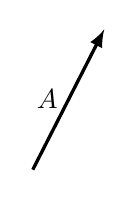
\begin{tikzpicture}
\draw[very thick, -latex] (0,0) -- (63:2) node[pos=0.5, left]{$\mat{A}$};
\end{tikzpicture}
\caption{}
\end{subfigure}\hfill
\begin{subfigure}{0.3\textwidth}
\centering
\begin{tikzpicture}
\draw[-latex] (0,0) -- (0,2.25)coordinate(ytip) node[left]{$y$};
\draw[-latex] (0,0) -- (2,0)coordinate(xtip) node[below]{$x$};
\draw[-latex, very thick] (0,0) -- (1,2)coordinate(atip) node[pos=0.4,right]{$\mat{A}$};
\draw[dashed](atip)--($(0,0)!(atip)!(xtip)$)coordinate(xi);
\draw[dashed](atip)--($(0,0)!(atip)!(ytip)$)coordinate(yi);
\draw (0.5,0) node[below]{$A_x$};
\draw (0,1.3) node[left]{$A_y$};
\draw (0.5,0) node[below]{$A_x$};
\end{tikzpicture}
\caption{}
\end{subfigure}\hfill
\begin{subfigure}{0.3\textwidth}
\centering
\begin{tikzpicture}
\draw [-latex] (0,0) -- (20:3)coordinate(xtip) node[below right]{$x'$};
\draw [-latex] (0,0) -- (110:3)coordinate(ytip) node[above right]{$y'$};
\draw[very thick, -latex] (0,0) -- (65:2.6)coordinate(a) node[pos=0.5, above left]{$\mat{A}$};
\draw[dashed] (a) -- ($(0,0)!(a)!(xtip)$)coordinate(xi);
\draw[dashed] (a) -- ($(0,0)!(a)!(ytip)$)coordinate(yi);
\draw($(0,0)!0.5!(xi)$)node[below right]{$A_{x'}$};
\draw($(0,0)!0.5!(yi)$)node[left]{$A_{y'}$};
\end{tikzpicture}
\caption{}
\end{subfigure}
\caption{
(ا) سمتیہ \عددی{\mat{A}}، (ب) \عددی{xy} محدد سے لحاظ سے \عددی{\mat{A}} کے اجزاء، (ج) \عددی{x'y'} محدد کے لحاظ سے \عددی{\kvec{A}} کے اجزاء
}
\label{شکل_قواعد_سمتیہ_کے_اجزاء}
\end{figure}


 یہی کچھ کوانٹم میکانیات میں ایک نظام کے حال کے لیے درست ہو گا۔ اس کو سمتیہ \عددی{| \s(t) \rangle } سے ظاہر کیا جا سکتا ہے جو "باہر ہلبرٹ فضا" میں رہتا ہے اور جسے ہم مختلف اساس کے لحاظ سے بیان کر سکتے ہیں۔ درحقیقت امتیازی تفاعل مقام کی اساس میں \عددی{| \s \rangle} کی پھیلاو کا عددی سر موجی تفاعل \عددی{\Psi(x,t)} ہو گا:
\begin{align}
\Psi(x,t) = \langle x | \s(t) \rangle 
\end{align}
(جہاں \عددی{\hat{x}} کے امتیازی تفاعل جس کی امتیازی قیمت \عددی{x} ہے کو سمتیہ \عددی{| x \rangle} ظاہر کرتا ہے) \حاشیہد{میں اس کو \عددی{g_x} (مساوات \حوالہ{مساوات_قواعد_ڈیراک_استعمال}) نہیں کہنا چاہتا چونکہ وہ اس کی اساس مقام میں روپ ہے، اور یہاں پورا مقصد کسی بھی مخصوص اساس سے چھٹکارا ہے۔ یقیناً میں نے پہلی مرتبہ ہلبرٹ فضا کو، \عددی{x} پر ، بطور   مربع متکامل  تفاعلات کا سلسلہ متعارف کرتے ہوئے اس کو (اساس مقام کا) پابند بنایا جو ایک امتناعی صورت ہے۔میں چاہتا ہوں کہ آپ اس کو ایک تصوراتی سمتی فضا سمجھیں، جس کے ارکان کو کسی بھی اساس کے لحاظ سے ظاہر کیا جا سکتا ہے۔ }، جبکہ معیار حرکت امتیازی تفاعل کی اساس میں \عددی{| \s \rangle } کی پھیلاو، مقام و معیار حرکت موجی تفاعل \عددی{\Phi(p,t)} ہے:
\begin{align}
\Phi(p,t) = \langle p | \s (t) \rangle
\end{align}
(جہاں \عددی{\hat{p}} کا امتیازی تفاعل جس کی امتیازی قیمت \عددی{ p} ہے کو سمتیہ \عددی{| p \rangle } ظاہر کرتا ہے)۔\حاشیہد{مقامی فضا میں یہ \عددی{f_p(x)} ہو گا (مساوات \حوالہ{مساوات_قواعد_امتیازی_تفاعل_معیار_حرکت})۔} ہم \عددی{| \s \rangle} کے پھیلاو کو توانائی امتیازی تفاعل کی اساس میں بھی کر سکتے ہیں (یہاں اپنی آسانی کے لیے ہم غیر مسلسل طیف فرض کر رہے ہیں) :
\begin{align}
c_{n} (t) = \langle n | \s (t) \rangle
\end{align}
(جہاں \عددی{\hat{H}} کے \عددی{n} ویں امتیازی تفاعل کو سمتیہ \عددی{| n \rangle } ظاہر کرتا ہے)؛ مساوات \حوالہ{مساوات_قواعد_فوریئر_ترکیب_عددی_سر}۔ تاہم یہ تمام ایک ہی حالت کو ظاہر کرتے ہیں؛ تفاعلات \عددی{\Psi} اور \عددی{\Phi}، اور عددی سروں کا سلسلہ \عددی{\{ c_{n} \} }ٹھیک ایک جیسی معلومات رکھتے ہیں؛ یہ ایک ہی سمتیہ کو ظاہر کرنے کے تین مختلف طریقے ہیں:
\begin{align}
\Psi (x,t) &= \int \Psi(y,t) \delta (x-y) \dif y = \int \Phi (p,t) \frac{1}{\sqrt{2\pi\hslash}} e^{ipx/\hslash} \dif p \nonumber \\ 
&= \sum c_{n} e^{-iE_{n}t/\hslash} \psi_{n}(x)
\end{align}
(قابل مشاہدہ کو ظاہر کرنے والے ) عاملین خطی مبدل ہوتے ہیں جو ایک سمتیہ کا "تبادلہ" دوسری سمتیہ میں کرتے ہیں۔
\begin{align}\label{مساوات_قواعد_بیٹا_سمتیہ}
| \beta \rangle = \hat{Q}|\alpha \rangle
\end{align}
بالکل سمتیات کی طرح جنہیں ایک مخصوص اساس \عددی{\{ |e_{n} \rangle \} }، \حاشیہد{میں فرض کرتا ہوں کہ یہ اساس غیر مسلسل ہے؛ مسلسل اساس کی صورت میں \عددی{n} استمراری ہو گا اور مجموعات کی جگہ تکملات ہوں گے۔} کے لحاظ سے ان کے اجزاء 
\begin{gather}
\begin{aligned}
\text{\RL{ہے، اور }}\quad a_{n} = \langle e_{n} | \alpha \rangle \quad \text{\RL{جہاں}}\quad | \alpha \rangle = \sum_{n} a_{n} | e_{n} \rangle \\
\text{\RL{ہے}}\quad b_{n} \langle e_{n} \beta \rangle\quad \text{\RL{جہاں}}\quad | \beta \rangle = \sum_{n} b_{n} | e_{n} \rangle
\end{aligned}
\end{gather}
سے ظاہر کیا جاتا ہے، عاملین کو( کسی مخصوص اساس کے لحاظ سے) ان کے \اصطلاح{قالبی ارکان}\فرہنگ{قالبی ارکان}\حاشیہب{matrix elements}\فرہنگ{matrix elements} \حاشیہد{یہ اصطلاح متناہی ابعادی صورت سے متاثر ہو کر منتخب کی گئی ہے، تاہم اس "قالب" کے اراکین کی تعداد اب لامتناہی ہو گی (جن کی گنتی نا ممکن بھی ہو سکتی ہے ) ۔}
\begin{align}
\langle e_{m} | \hat{Q} | e_{n}\rangle \equiv Q_{mn}
\end{align}
سے ظاہر کیا جاتا ہے ۔ اس علامت کو استعمال کرتے ہوئے مساوات \حوالہ{مساوات_قواعد_بیٹا_سمتیہ} درج ذیل روپ اختیار کرتی ہے 
\begin{align}
\sum_{n} b_{n} | e_{n} \rangle = \sum_{n} a_{n} \hat{Q} | e_{n} \rangle
\end{align}
یا، سمتیہ \عددی{| e_{m} \rangle} کے ساتھ اندرونی ضرب لیتے ہوئے 
\begin{align}
\sum_{n} b_{n} \langle e_{m} | e_{n} \rangle = \sum_{n} a_{n} \langle e_{m} | \hat{Q} | e_{n} \rangle
\end{align}
لہٰذا درج ذیل ہو گا ۔
\begin{align}
b_{m} = \sum_{n} Q_{mn}a_{n}
\end{align}
یوں اجزاء کے تبادلہ کے بارے میں قالبی ارکان معلومات فراہم کرتے ہے ۔

بعد میں ہمیں ایسے نظاموں سے واسطہ ہو گا جن کے خطی غیر تابع حالات کی تعداد متناہی عدد \عددی{(N)} ہو گا۔سمتیہ \عددی{| \s (t) \rangle} ایسی صورت میں \عددی{N} ابعادی سمتی فضا میں رہتا ہے؛ جس کو (کسی دیے گئے اساس کے لحاظ سے)، \عددی{(N)} اجزاء کی قطار سے ظاہر کیا جا سکتا ہے جبکہ عاملین \عددی{(N \times N)} سادہ قالب کا روپ اختیار کرتے ہیں۔ یہ سادہ ترین کوانٹائی نظام ہیں؛ جن میں لامتناہی آبادی سمتی فضا سے وابستہ باریکیاں نہیں پائی جاتی ہیں۔ ان میں سب سے آسان دو حالتی نظام ہے جس پر درج ذیل مثال میں غور کیا گیا ہے۔

% Example 3.8
\ابتدا{مثال}
تصور کریں کہ ایک نظام میں صرف دو (درج ذیل) خطی غیر تابع حالات ممکن ہیں۔\حاشیہد{یہاں "مساوات" کی نشان سے مراد "ظاہر کرتا ہے" لینا چاہیے، تاہم میرے خیال میں اس غیر رسمی علامتیت کے استعمال سے غلط فہمی پیدا ہونے کا کوئی امکان نہیں پایا جاتا ہے۔} 
\begin{align*}
 |2\rangle = \begin{pmatrix} 0 \\ 1 \end{pmatrix}\quad \text{اور}\quad |1\rangle = \begin{pmatrix} 1 \\ 0 \end{pmatrix}
\end{align*}
سب سے زیادہ عمومی حال ان کا معمول شدہ خطی جوڑ 
\begin{align*}
 \text{\RL{ہے۔}}\quad |a|^{2} + |b|^{2} = 1\quad \text{\RL{ہو گا جہاں}}\quad | \s \rangle = a|1\rangle +b|2\rangle = \begin{pmatrix} a \\ b \end{pmatrix} 
\end{align*}
ہیملٹنی کو ایک (ہرمشی) قالب کے روپ میں لکھا جا سکتا ہے؛ فرض کریں کہ اس کا مخصوص روپ درج ذیل ہے 
\begin{align*}
\mat{H} = \begin{pmatrix} h & g \\ g & h \end{pmatrix}
\end{align*}
جہاں\عددی{g} اور \عددی{h} حقیقی مستقل ہیں۔ اگر( \عددی{t=0} پر ) یہ نظام حال \عددی{|1\rangle} سے ابتدا کرے تب وقت \عددی{t} پر اس کا حال کیا ہو گا؟ 

\موٹا{حل:} \quad 
 (تابع وقت) شروڈنگر مساوات درج ذیل کہتی ہے۔ 
\begin{align}
i \hslash \frac{\dif}{\dif t} | \s \rangle = H | \s \rangle
\end{align}
ہمیشہ کی طرح ہم غیر تابع تابع شروڈنگر
\begin{align}
H | \s \rangle = E | \s \rangle 
\end{align}
 کے حل سے ابتداء کرتے ہیں، یعنی ہم \عددی{H} کی امتیازی سمتیات اور امتیازی اقدار تلاش کرتے ہیں۔ امتیازی اقدار کی قیمت امتیازی مساوات تعین کرتی ہے ۔
\begin{align*}
 \begin{pmatrix} h-E & g \\ g & h-E \end{pmatrix}\text{مقطع} = (h-E)^{2} - g^{2} = 0 \Rightarrow h-E = \mp g \Rightarrow E_{\pm} = h \pm g
\end{align*}
آپ دیکھ سکتے ہیں کہ اجازتی توانائیاں \عددی{( h+g)} اور \عددی{(h-g)} ہیں۔ امتیازی سمتیات تعین کرنے کی خاطر ہم درج ذیل لکھتے ہیں 
\begin{align*}
\begin{pmatrix} h & g \\ g & h \end{pmatrix} \begin{pmatrix}
 \alpha \\ \beta \end{pmatrix} = (h\pm g) \begin{pmatrix} \alpha \\ \beta \end{pmatrix} \Rightarrow h\alpha + g\beta = (h\pm g) \alpha \Rightarrow \beta = \pm \alpha
\end{align*}
لہٰذا معمول شدہ امتیازی سمتیات درج ذیل ہوں گے ۔
\begin{align*}
| \s _{\pm} \rangle = \frac{1}{\sqrt{2}} \begin{pmatrix} 1 \\ \pm 1 \end{pmatrix}
\end{align*}
اس کے بعد ابتدائی حال کو ہم ہیملٹنی کے امتیازی سمتیات کے خطی جوڑ کی صورت میں لکھتے ہیں ۔
\begin{align*}
| \s (0) \rangle = \begin{pmatrix} 1 \\ 0 \end{pmatrix} = \frac{1}{\sqrt{2}} ( | \s_{+} \rangle + | \s_{-} \rangle )
\end{align*}
آخر میں ہم اس کے ساتھ معیاری تابعیت وقت جزو \عددی{e^{-iE_{n}t/\hslash}} منسلک کرتے ہیں۔ 
\begin{align*}
| \s (t) \rangle &= \frac{1}{\sqrt{2}} [ e^{-i(h+g)t/\hslash} | \s_{+} \rangle + e^{-i(h-g)t/\hslash} | \s_{-} \rangle ] \\
&= \frac{1}{2} e^{-iht/\hslash} \Big[ e^{-igt/\hslash} \begin{pmatrix} 1 \\ 1 \end{pmatrix} + e^{igt/\hslash} \begin{pmatrix} 1 \\ -1 \end{pmatrix} \Big] \\
&= \frac{1}{2} e^{-iht/\hslash} \begin{pmatrix} e^{-igt/\hslash} + e^{igt/\hslash} \\ e^{-igt/\hslash} - e^{igt/\hslash} \end{pmatrix} = e^{-iht/\hslash} \begin{pmatrix} \cos (gt/\hslash) \\ -i\sin (gt/\hslash) \end{pmatrix}
\end{align*}
اگر آپ کو اس نتیجے پر شک ہو تو آپ اس کی جانچ پڑتال کر سکتے ہیں: کیا یہ تابع وقت شروڈنگر مساوات کو مطمئن کرتا ہے؟ کیا یہ \عددی{t=0} پر ابتدائی حال کے موافق ہے؟ 

یہ (دیگر چیزوں کے علاوہ ) \اصطلاح{ ارتعاش نیوٹرینو}\فرہنگ{ارتعاش!نیوٹرینو}\حاشیہب{neutrino oscillations}\فرہنگ{oscillation!neutrino} کا ایک سادہ نمونہ ہے جہاں \عددی{|1\rangle}\اصطلاح{ الیکٹران نیوٹرینو}\فرہنگ{الیکٹران نیوٹرینو}\حاشیہب{electron neutrino}\فرہنگ{neutrino!electron} ، اور \عددی{|2\rangle}\اصطلاح{ میون نیوٹرینو}\فرہنگ{میون نیوٹرینو}\حاشیہب{muon neutrino}\فرہنگ{neutrino!muon} کو ظاہر کرتا ہے؛ اگر ہیملٹنی میں خلاف وتر جزو \عددی{(g)} غیر معدوم ہو تب وقت گزرنے کے ساتھ بار بار الیکٹران نیوٹرینو تبدیل ہو کر میون نیوٹرینو میں اور میون نیوٹرینو واپس الیکٹران نیوٹرینو میں تبدیل ہوتا رہے گا۔
\انتہا{مثال}


کوانٹم  میکانیات میں اندرونی ضرب کو \اصطلاح{ڈیراک علامتیت}\فرہنگ{ڈیراک!علامتیت}\حاشیہب{Dirac notation}\فرہنگ{Dirac!notation} سے ظاہر کیا جاتا ہے جو   تکونی  قوسین، \عددی{\langle} اور \عددی{\rangle}، اور افقی لکیر \عددی{|}،    پر مشتمل  ہے۔ یوں  کوانٹم میکانیات میں  تکونی  قوسین  کو قوسین نہیں بلکہ عاملین تصور کریں۔ اندرونی ضرب   \عددی{ \langle \alpha | \beta \rangle}  کو  دو حصوں   \عددی{\langle \alpha|} اور \عددی{|\beta\rangle} میں تقسیم کیا جاتا ہے جنہیں بالترتیب \اصطلاح{تفاعلیہ}\فرہنگ{تفاعلیہ}\حاشیہب{bra}\فرہنگ{bra} اور \اصطلاح{سمتاویہ}\فرہنگ{سمتاویہ}\حاشیہب{ket}\فرہنگ{ket} کہتے ہیں۔  ان میں سے موخر الذکر ایک سمتیہ ہے، مگر اول الذکر کیا ہے؟ یہ اس لحاظ سے سمتیات کا ایک \ترچھا{ خطی تفاعل} ہے کہ اس کے دائیں جانب ایک سمتیہ  چسپاں کرنے  سے ایک( مخلوط) عدد حاصل ہوتا ہے جو اندرونی ضرب ہو گا۔( ایک عامل کے ساتھ سمتیہ چسپاں  کرنے  سے دوسرا سمتیہ حاصل ہوتا ہے جبکہ ایک  تفاعلیہ کے ساتھ سمتیہ  چسپاں   کرنے سے ایک عدد حاصل ہوتا ہے۔) جیسا آپ دیکھیں گے کوانٹم  میکانیات میں  تفاعلیہ کو ایک قالب اور سمتاویہ کو سمتیہ کی روپ میں لکھا جاتا ہے۔ ڈیراک علامتیت کو \اصطلاح{تفاعلیہ و سمتاویہ علامتیت}\فرہنگ{علامتیت!تفاعلیہ و سمتاویہ}\حاشیہب{bra-ket notation}\فرہنگ{bra-ket!notation} بھی کہتے ہیں۔ ایک تفاعلی فضا میں تفاعلیہ  کو تکمل لینے کی ہدایت تصور کیا جا سکتا ہے:
\begin{align*}
\langle f | = \int f^{*} [ \cdots ] \dif x
\end{align*}
جہاں چوکور  قوسین \عددی{[\cdots]} میں وہ تفاعل پر کیا جائے گا جو تفاعلیہ کے دائیں ہاتھ سمتاویہ میں موجود ہو گا۔ ایک متناہی ابعاد سمتی فضا میں، جہاں سمتیات کو قطاروں 
\begin{align}
| \alpha \rangle = \begin{pmatrix}
a_{1} \\ a_{2} \\ \vdots \\ a_{n} 
\end{pmatrix}
\end{align}
کی صورت میں بیان کیا گیا ہو، مطابقتی تفاعلیہ ایک سمتیہ صف 
\begin{align}
\langle \alpha | = ( a_{1}^{*}a_{2}^{*} \dotsc a_{n}^{*})
\end{align}
ہو گا۔ تمام تفاعلیہ کو اکٹھا کرنے سے دوسرا سمتی فضا حاصل ہو گا جس کو \اصطلاح{ دوہری فضا }\فرہنگ{فضا!دوہری}\حاشیہب{dual space}\فرہنگ{space!dual}کہتے ہیں۔ 

تفاعلیہ کی ایک علیحدہ وجود کا تصور ہمیں طاقتور اور خوبصورت علامتیت کا موقع فراہم کرتی ہے( اگرچہ اس کتاب میں اس سے فائدہ نہیں اٹھایا جائے گا) ۔ مثال کے طور پر، اگر \عددی{| \alpha \rangle} ایک معمول شدہ سمتیہ ہو، تب عامل 
\begin{align}
\hat{P} \equiv | \alpha \rangle \langle \alpha | 
\end{align}
کسی بھی دوسرے سمتیہ کا وہ حصہ اٹھاتا (منتخب کرتا) ہے جو \عددی{ | \alpha \rangle} کے"ساتھ ساتھ" پایا جاتا ہو:
\begin{align*}
\hat{P} | \beta \rangle = \langle \alpha | \beta \rangle | \alpha \rangle ;
\end{align*}
ہم اس کو \عددی{| \alpha \rangle} کے احاطہ کیے گئے یک بعدی ذیلی فضا پر \اصطلاح{عامل تظلیل}\فرہنگ{عامل!تظلیل}\حاشیہب{projection operator}\فرہنگ{operator!projection} کہتے ہیں۔ اگر \عددی{\{ | e_{n} \rangle\} } غیر مسلسل معیاری عمودی اساس،
\begin{align}
\langle e_{m} | e_{n} \rangle = \delta_{mn}
\end{align}
ہو تب درج ذیل ہو گا 
\begin{align}\label{مساوات_قواعد_مکملیت_الف}
\sum_{n} | e_{n} \rangle \langle e_{n} | = 1 
\end{align}
(جو عامل مماثل ہے)۔ چونکہ کسی بھی سمتیہ \عددی{| \alpha \rangle} پر عمل کرتے ہوئے یہ عامل اساس\عددی{\{ |e_{n} \rangle \}} میں سمتیہ \عددی{| \alpha \rangle} کے پھیلاو کو دوبارہ سے حاصل کرتا ہے۔ 
\begin{align}
\sum_{n} | e_{n} \rangle \langle e_{n} | \alpha \rangle = | \alpha \rangle 
\end{align}
اسی طرح اگر \عددی{\{ | e_{z} \rangle \}} ڈیراک معیاری عمود شدہ استمراری اساس 
\begin{align}
\langle e_{z} | e_{z^{'}} \rangle = \delta ( z-z^{'})
\end{align}
ہو، تب درج ذیل ہو گا۔ 
\begin{align}\label{مساوات_قواعد_مکملیت_ب}
\int | e_{z} \rangle \langle e_{z} | \dif z = 1
\end{align}
 مساوات \حوالہ{مساوات_قواعد_مکملیت_الف} اور مساوات \حوالہ{مساوات_قواعد_مکملیت_ب} مکملیت کو خوش اسلوبی سے بیان کرتے ہیں۔
 
 
% Problem 3.21 
\ابتدا{سوال}
دکھائیں کہ عاملین تظلیل \اصطلاح{یک طاقتی}\فرہنگ{یک طاقتی}\حاشیہب{idempotent}\فرہنگ{idempotent} ہیں، یعنی ان کے لئے \عددی{\hat{P}^{2} = \hat{P}}ہو گا۔ \عددی{\hat{P}} کے امتیازی اقدار تعین کریں اور اس کے امتیازی سمتیات کے خواص بیان کریں۔
\انتہا{سوال}
% Problem 3.22
\ابتدا{سوال}
 معیاری عمودی اساس \عددی{| 1 \rangle }، \عددی{| 2 \rangle } ، \عددی{| 3 \rangle } کا احاطہ کیے گئے تین بعدی فضا پر غور کریں۔سمتاویہ \عددی{| \alpha \rangle } اور  سمتاویہ \عددی{| \beta \rangle } درج ذیل ہیں۔ 
\begin{align*}
| \alpha \rangle = i | 1 \rangle -2|2\rangle -i|3\rangle , \quad | \beta \rangle = i|1\rangle +2|3\rangle 
\end{align*}
\begin{enumerate}[a.]
\item
 \عددی{ \langle \alpha |} اور \عددی { \langle \beta |} کو ( دوہری اساس \عددی{\langle 1 |} ،\عددی{ \langle 2 |}، \عددی{ \langle 3 |} کی صورت میں) تیار کریں۔ 
\item
 \عددی{ \langle \alpha | \beta \rangle} اور \عددی{ \langle \beta | \alpha \rangle} تلاش کریں اور \عددی{ \langle \beta | \alpha \rangle = \langle \alpha | \beta \rangle^{*}} کی تصدیق کریں۔
\item
 اس اساس میں عامل \عددی{ \hat{A} \equiv | \alpha \rangle \langle \beta | } کے نو ارکان قالب تلاش کر کے قالب \عددی{\mat{A}} تیار کریں۔ کیا یہ ہرمشی ہے؟
\end{enumerate} 
\انتہا{سوال}
% Problem 2.23
\ابتدا{سوال}
کسی دو سطحی نظام کا ہیملٹنی درج ذیل ہے 
\begin{align*}
\hat{H} = E( | 1 \rangle \langle 1 | - |2\rangle \langle 2 | + | 1 \rangle \langle 2 | + | 2 \rangle \langle 1 | )
\end{align*}
جہاں \عددی{ | 1 \rangle , | 2 \rangle } معیاری عمودی اساس اور \عددی{ E} ایسا عدد ہے جس کا بعد توانائی کا ہے۔ اس کے امتیازی اقدار اور ( \عددی{| 1 \rangle } اور \عددی{| 2 \rangle } کے خطی جوڑ کی صورت میں معمول شدہ) امتیازی تفاعل تلاش کریں۔ اس اساس کے لحاظ سے \عددی{\hat{H}} کا قالب \عددی{\mat{H}} کیا ہو گا؟ 
\انتہا{سوال}
%Problem 2.24
\ابتدا{سوال}
 فرض کریں عامل \عددی{\hat{Q}} کے معیاری عمودی امتیازی تفاعلات کا ایک مکمل سلسلہ درج ذیل ہے۔ 
\begin{align*}
\hat{Q}|e_{n} \rangle = q_{n} | e_{n} \rangle \quad (n = 1,2,3,\dotsc )
\end{align*}
دکھائیں کہ \عددی{\hat{Q}} کو اس کے\اصطلاح{ طیفی تحلیل}\فرہنگ{طیفی تحلیل}\حاشیہب{spectral decomposition}\فرہنگ{decomposition!spectral}
\begin{align*}
\hat{Q} = \sum_{n} q_{n} | e_{n} \rangle \langle e_{n} |
\end{align*}
 کی صورت میں لکھا جا سکتا ہے ۔ \ترچھا{اشارہ:} \quad 
 تمام ممکنہ سمتیات پر عامل کے عمل سے عامل کو جانچا جاتا ہے لہٰذا کسی بھی سمتیہ \عددی{| \alpha \rangle} کے لیے آپ کو درج ذیل دکھانا ہو گا۔ 
\begin{align*}
\hat{Q} | \alpha \rangle = \left\{ \sum_{n} q_{n} | e_{n} \rangle \langle e_{n} | \right\} | \alpha \rangle 
\end{align*}
\انتہا{سوال}

\حصہء{مزید سوالات برائے باب \حوالہ{باب_قواعد_و_ضوابط}}
\ابتدا{سوال}
\موٹا{لیژانڈر کثیر رکنیاں۔} وقفہ \عددی{-1 \leq x \leq 1} پر تفاعلات \عددی{1}، \عددی{x}، \عددی{x^2} اور \عددی{x^{3}} کو گرام و شمد طریقہ کار سے معیاری عمود بنائیں( سوال \حوالہء{A. 4} دیکھیں) ۔عین ممکن ہے کہ آپ نتائج کو پہچان پائیں؛ (معیاری عمود زنی کے علاوہ)\حاشیہد{لیژانڈر کو معلوم نہیں تھا کہ کونسی روایت بہتر ثابت ہو گی۔ انہوں نے مجموعی جزو ضربی یوں منتخب کیا کہ \عددی{x=1} پر تمام تفاعلات \عددی{1} کے برابر ہوں؛ ہم اس بد قسمت انتخاب کی پیروی کرنے پر مجبور ہیں ۔} یہ لیژانڈر کثیر رکنیاں ہیں (جدول \حوالہ{جدول_ابعاد_لیژانڈر_چند_ابتدائی})۔
\انتہا{سوال}
\ابتدا{سوال}\شناخت{سوال_قواعد_مزید_خلاف_ہرمشی}
% Problem 3.26
ایک \اصطلاح{خلاف ہرمشی}\فرہنگ{ہرمشی!خلاف}\حاشیہب{anti-hermitian}\فرہنگ{hermitian!anti}( یا \اصطلاح{منحرف ہرمشی}\فرہنگ{ہرمشی!منحرف}\حاشیہب{skew-hermitian}\فرہنگ{hermitian!skew}) عامل اپنے ہرمشی جوڑی دار کا \ترچھا{منفی} ہوتا ہے۔ 
 \begin{align}
 \hat{Q}^{\dagger} = -\hat{Q}
 \end{align}
\begin{enumerate}[a.]
\item
 دکھائیں کہ خلاف ہرمشی عامل کی توقعاتی قیمت خیالی ہو گی۔
\item
 دکھائیں کہ دو عدد ہرمشی عاملین کا مقلب خلاف ہرمشی ہو گا۔ دو عدد خلاف ہرمشی عاملین کے مقلب کے بارے میں کیا کہا جا سکتا ہے؟ 
\end{enumerate}
\انتہا{سوال}
\ابتدا{سوال}
% Problem 3.27
\اصطلاح{ترتیبی پیمائشیں}\فرہنگ{ترتیبی پیمائشیں}\حاشیہب{sequential measurements}\فرہنگ{sequential measurements}: \quad
قابل مشاہدہ \عددی{A} کو ظاہر کرنے والے عامل \عددی{\hat{A}} کے دو معمول شدہ امتیازی حالات \عددی{\psi_{1}}اور \عددی{\psi_{2}}، جن کے امتیازی اقدار بالترتیب \عددی{a_{1}}اور \عددی{a_{2}}ہیں، پائے جاتے ہیں ۔ قابل مشاہدہ \عددی{B} کو ظاہر کرنے والے عامل \عددی{\hat{B}} کے دو معمول شدہ امتیازی حالات \عددی{\phi_{1}}اور \عددی{\phi_{2}} اور بالترتیب امتیازی اقدار \عددی{b_{1}}اور \عددی{b_{2}} ہیں۔ ان امتیازی حالات کا تعلق درج ذیل ہے۔ 
\begin{align*}
\psi_{1} = ( 3\phi_{1} + 4\phi_{2})/5, \quad \psi_{2} = ( 4\phi_{1} - 3\phi_{2})/5
\end{align*}
\begin{enumerate}[a.]
\item 
 قابل مشاہدہ \عددی{ A} کی پیمائش \عددی{ a_{1} } قیمت دیتی ہے۔اس پیمائش کے( فوراً) بعد یہ نظام کس حال میں ہو گا؟ 
\item
 اب اگر \عددی{ B} کی پیمائش کی جائے تو کیا نتائج ممکن ہوں گے اور ان کے احتمال کیا ہوں گے؟ 
\item
 قابل مشاہدہ \عددی{ B} کی پیمائش کے فوراً بعد دوبارہ \عددی{ A} کی پیمائش کی جاتی ہے ۔نتیجہ \عددی{ a_{1}} حاصل کرنے کا احتمال کیا ہو گا؟ ( دھیان رہے کہ اگر میں آپ کو \عددی{ B} کی پیمائش کا نتیجہ بتاتا تب جواب بہت مختلف ہوتا۔) 
\end{enumerate}
\انتہا{سوال}
\ابتدا{سوال}
% Problem 3.28
لامتناہی چوکور  کنویں کے \عددی{n} ویں ساکن حال کی معیار حرکت و فضا تفاعل موج \عددی{\Phi_{n}(p,t)} تلاش کریں۔ \عددی{| \Phi_{1}(p,t) |^{2}}اور \عددی{| \Phi_{2}(p,t) |^{2}} کو \عددی{p} کے تفاعل کے طور پر ترسیم کریں (نقاط \عددی{p = \pm n\pi\hslash/a} پر خصوصی توجہ دیں)۔ \عددی{\Phi_{n}(p,t)} کو استعمال کرتے ہوئے \عددی{p^{2}} کی توقعاتی قیمت کا حساب لگائیں۔ اپنے جواب کا سوال \حوالہ{سوال_غیر_تابع_لامتناہی_این_ویں} کے ساتھ موازنہ کریں۔
\انتہا{سوال}
\ابتدا{سوال}
% Problem 3.29
درج ذیل تفاعل موج پر غور کریں
\begin{align*}
\Psi(x,0) = 
\begin{cases}
\frac{1}{\sqrt{2n\lambda}}e^{i2\pi x/\lambda}, & -n\lambda < x < n \lambda \\ 
0, & \text{\RL{دیگر صورت}}
\end{cases}
\end{align*}
جہاں \عددی{n} کوئی مثبت عدد صحیح ہے۔ اگرچہ وقفہ \عددی{-n\lambda < x < n \lambda} پر یہ تفاعل خالص سائن نما ہے( جس کا طول موج \عددی{\lambda} ہے) تاہم چونکہ یہ تفاعل لامتناہی تک ارتعاش جاری نہیں رکھتا لہٰذا اس کی معیار حرکت کی قیمتیں ایک سعت پر مشتمل ہوں گی۔اس کا معیار حرکت و فضا تفاعل موج \عددی{\Phi(p,0)} تلاش کریں۔ \عددی{| \Psi(x,0)|^{2}}اور \عددی{| \Phi(p,0)|^{2}} ترسیم کر کے ( مرکزی چوٹی کے اطراف صفروں کے بیچ) چوڑائیاں \عددی{\omega_{x}}اور \عددی{\omega_{p}} تعین کریں۔ دیکھیں کہ \عددی{n \rightarrow \infty} کا ان چوڑائیوں پر کیا اثر ہو گا؟ \عددی{\omega_{x}} اور \عددی{\omega_{p}} کو \عددی{\Delta x}اور \عددی{\Delta p} کی اندازاً قیمتیں لیتے ہوئے تصدیق کریں کہ اصول عدم یقینیت مطمئن ہوتا ہے۔ \ترچھا{انتباہ:} اگر آپ \عددی{\sigma_{p}} کا حساب کرنے کی کوشش کریں تو آپ کو حیرانی کا سامنا ہو گا۔ کیا آپ اس مسئلے کی وجہ بتلا سکتے ہیں؟ 
\انتہا{سوال}
\ابتدا{سوال}
% Problem 3.30
درج ذیل فرض کریں
\begin{align*}
\Psi(x,0) = \frac{A}{x^{2}+a^{2}} 
\end{align*}
جہاں \عددی{A} اور \عددی{a} مستقلات ہیں۔
\begin{enumerate}[a.]
\item
 \عددی{ \Psi(x,0)}کو معمول پر لاتے ہوئے \عددی{A} تعین کریں ۔
\item
 (لمحہ \عددی{ t=0 } پر) \عددی{\langle x \rangle}، \عددی{ \langle x^{2} \rangle}اور \عددی{ \sigma_{x} } تلاش کریں۔
\item
 معیار حرکت و فضا تفاعل موج \عددی{ \Phi(p,0)} تلاش کریں اور تصدیق کریں کہ یہ معمول شدہ ہے۔
\item
 \عددی{ \Phi(p,0) }استعمال کرتے ہوئے (لمحہ \عددی{ t=0} پر) \عددی{ \langle p \rangle } \عددی{ \langle p^{2} \rangle}اور \عددی{ \sigma_{p} } کا حساب کریں ۔
\item
 اس حال کے لیے ہیزنبرگ اصول عدم یقینیت کو جانچیں۔ 
\end{enumerate}
\انتہا{سوال}
\ابتدا{سوال}\شناخت{سوال_قواعد_مسئلہ_وریل}\موٹا{مسئلہ وریل۔}\quad
%Problem 3.31
 درج ذیل مساوات \حوالہ{مساوات_قواعد_شرح_تبدیلی_قابل_مشاہدہ} کی مدد سے دکھائیں 
\begin{align}
\frac{\dif}{\dif t} \langle xp \rangle -2\langle T \rangle - \big\langle x \frac{\dif V}{\dif x} \big\rangle
\end{align}
جہاں \عددی{ T} حرکی توانائی \عددی{( H=T+V ) } ہے۔\ترچھا{ ساکن} حال میں بایاں ہاتھ صفر ہو گا( ایسا کیوں ہے؟) لہٰذا درج ذیل ہو گا ۔
\begin{align}
2\langle T \rangle = \big\langle x \frac{\dif V}{\dif x} \big\rangle
\end{align}
اس کو \اصطلاح{مسئلہ وریل}\فرہنگ{مسئلہ وریل}\حاشیہب{virial theorem}\فرہنگ{virial theorem} کہتے ہیں۔ ہارمونی مرتعش کے ساکن حالات کے لیے اس مسئلہ کو استعمال کرتے ہوئے ثابت کریں کہ \عددی{ \langle T \rangle = \langle V \rangle } ہو گا اور تصدیق کریں کہ یہ سوال\حوالہ{سوال_غیر_تابع_وقت_صریح_تکملات} اور سوال \حوالہ{سوال_شروڈنگر_تصدیق_کریں} میں آپ کے نتائج کے ہم آہنگ ہے۔
\انتہا{سوال}
%126-128
% example 3.32
\ابتدا{سوال} 
توانائی و وقت کی عدم یقینیت کے اصول کا ایک دلچسپ روپ \عددی{\Delta t=\tau/\pi} ہے جہاں ابتدائی حال \عددی{\Psi (x,0)} کے عمودی حال تک \عددی{\Psi(x,t)} کی ارتقا کے لیے درکار وقت \عددی{\tau} ہے۔ دو (معیاری عمودی) ساکن حالات کے برابر حصوں پر مشتمل ( اختیاری) مخفیہ کا تفاعل موج \عددی{\Psi(x,0)=1/\sqrt{2}[\psi_{1}(x)+\psi_{2}(x)]} استعمال کرتے ہوئے اس کی چانچ پڑتال کریں۔
\انتہا{سوال}

\ابتدا{سوال} 
%3.33\\
ہارمونی مرتعش کے ساکن حالات کی (معیاری عمودی) اساس (مساوات \حوالہ{مساوات_شروڈنگر_ہارمونی_ساکن_حالات}) میں قالبی ارکان \عددی{\langle n|x|n'\rangle} اور \عددی{\langle n|p|n'\rangle} تلاش کریں۔ آپ سوال \حوالہ{سوال_شروڈنگر_تصدیق_کریں} میں قالبی وتری رکن \عددی{n=n'} دریافت کر چکے ہیں؛ وہی ترکیب موجودہ عمومی مسئلے میں استعمال کریں۔ متعلقہ( لامتناہی) قالب \عددی{\mat{X}} اور \عددی{\mat{P}}  مرتب کریں۔ دکھائیں کہ اس اساس میں
\عددی{\tfrac{1}{2m}\mat{P}^2+\tfrac{m\omega^2}{2}\mat{X}^2=\mat{H}}\ترچھا{ وتری} ہو گا۔ کیا اس کے وتر ی ارکان آپ کے توقع کے مطابق ہیں؟
\ترچھا{جزوی جواب:} 
\begin{align}
\langle n|x|n'\rangle=\sqrt{\frac{\hslash}{2m\omega}}(\sqrt{n'}\delta_{n,n'-1}+\sqrt{n}\delta_{n',n-1})
\end{align}
\انتہا{سوال}

\ابتدا{سوال}
ایک ہارمونی مرتعش ایسے حال میں ہے کہ اس کی توانائی کی پیمائش، ایک  جتنے احتمال کے ساتھ، \عددی{(1/2)\hslash\omega} یا \عددی{(3/2)\hslash\omega} دے گی۔ اس حال میں \عددی{\langle p\rangle} کی زیادہ سے زیادہ ممکنہ قیمت کیا ہو گی؟ اگر لمحہ \عددی{t=0} پر اس کی قیمت (یہی زیادہ سے زیادہ قیمت) ہو تب \عددی{\Psi(x,t)} کیا ہو گا؟
\انتہا{سوال}

 \ابتدا{سوال} 
3۔35\\
\موٹا{ہارمونی مرتعش کے اتساقی حالات۔ } \quad ہارمونی مرتعش کے ساکن حالات ( \عددی{|n\rangle =\psi_{n}(x)}، مساوات \حوالہ{مساوات_شروڈنگر_ہارمونی_ساکن_حالات}) میں صرف \عددی{n=0} عین عدم یقینیت کی
 حد ( \عددی{\sigma_{x}\sigma_{p}=\hslash/2}) پر بیٹھتا ہے؛ جیسا آپ سوال \حوالہ{سوال_شروڈنگر_تصدیق_کریں} میں معلوم کر چکے ہیں عمومی طور پر \عددی{\sigma_{x}\sigma_{p}=(2n+1)\hslash/2} ہو گا۔ تاہم چند \ترچھا{خطی جوڑ} ( جنہیں\اصطلاح{ اتساقی حالات}\فرہنگ{اتساقی!حالات}\حاشیہب{coherent states}\فرہنگ{coherent states} کہتے ہیں) بھی عدم یقینیت کے حاصل ضرب کو کم سے کم بناتے ہیں۔ ہم دیکھتے ہیں کہ یہ \ترچھا{ عامل تقلیل}\حاشیہد{عامل رفعت کے ایسے امتیازی حالات جنہیں معمول پر لانا ممکن ہو نہیں پائے جاتے ہیں۔} کے \ترچھا{امتیازی تفاعل} ہوں گے
\begin{align*}
a_{-}|\alpha\rangle =\alpha|\alpha\rangle
\end{align*}
(جہاں امتیاز ی قدر \عددی{\alpha} کوئی بھی مخلوط عدد ہو سکتا ہے)۔
\begin{enumerate}[a.] 
\item
حال \عددی{|\alpha\rangle} میں \عددی{\langle x \rangle} ، \عددی{\langle x^{2} \rangle} ، \عددی{\langle p \rangle} ، \عددی{\langle p^{2} \rangle} دریافت کریں۔ \ترچھا{اشارہ:} مثال \حوالہ{مثال_شروڈنگر_ہارمونی_مرتعش_مخفی_توقعاتی} کی ترکیب استعمال کریں اور یاد رکھیں کہ \عددی{a_{-}} کا ہرمشی جوڑی دار \عددی{a_{+}} ہے۔ فرض نہ کریں کہ \عددی{\alpha} حقیقی ہو گا۔ 
\item
\عددی{\sigma_{x}} اور \عددی{\sigma_{p}} تلاش کریں۔ دکھائیں کہ \عددی{\sigma_{x}\sigma_{p}=\hslash/2} ہو گا ۔ 
\item
کسی بھی دوسرے تفاعل موج کی طرح، اتساقی حال کو توانائی امتیازی حالات کا پھیلاو 
 \begin{align*} 
|\alpha\rangle=\sum_{n=0}^{\infty}c_{n}|n\rangle 
 \end{align*} 
 لکھا جا سکتا ہے۔ دکھائیں کہ پھیلاو کے عددی سر درج ذیل ہونگے۔ 
 \begin{align*} 
c_{n}=\frac{\alpha^{n}}{\sqrt{n!}}c_{0} 
 \end{align*} 
\item
 \عددی{|\alpha\rangle} کو معمول پر لاتے ہوئے \عددی{c_{0}} تعین کریں۔\ترچھا{ جواب:} \عددی{e^{-\abs{\alpha}^2/2}} 
 \item
 اس کے ساتھ تابعیت وقت 
 \begin{align*} 
|n\rangle\to e^{-iE_{n}t/\hslash}|n\rangle 
 \end{align*} 
شامل کر کے دکھائیں کہ \عددی{|\alpha(t)\rangle} اب بھی \عددی{a{-}} کا امتیازی حال ہو گا، تاہم وقت کے ساتھ امتیازی قدر ارتقا پذیر ہو گا۔ 
 \begin{align*} 
\alpha(t)=e^{-i\omega t}\alpha 
 \end{align*} 
یوں اتساقی حال ہمیشہ اتساقی حال ہی رہے گا اور عدم یقینیت کے حاصل ضرب کو کم سے کم کرتا رہے گا۔ 
\item
کیا زمینی حال \عددی{|n=0\rangle} خود اتساقی حال ہو گا؟ اگر ایسا ہو تب امتیازی قدر کیا ہو گا۔
\end{enumerate}
 \انتہا{سوال}

\ابتدا{سوال} 
%3.36 
\موٹا{مبسوط اصول عدم یقینیت۔}\quad متعمم اصول عدم یقینیت (مساوات \حوالہ{مساوات_قواعد_عمومی_اصول_عدم_یقینیت_الف_بے}) درج ذیل کہتا ہے
 \begin{align*} 
\sigma_{A}^{2}\sigma_{B}^{2}\geq\frac{1}{4}\langle C^{2} \rangle 
 \end{align*} 
جہاں \عددی{\hat{C}\equiv -i[\hat{A},\hat{B}] } ہے۔
\begin{enumerate}[a.] 
\item
دکھائے کہ اس کو زیادہ مستحکم بنا کر درج ذیل روپ میں لکھا جا سکتا ہے
 \begin{align}\label{مساوات_سوال_مستحکم_عدم_یقینیت} 
\sigma_{A}^{2}\sigma_{B}^{2}\geq\frac{1}{4}(\langle C\rangle^{2}+\langle D \rangle ^{2}) 
 \end{align} 
جہاں \عددی{\hat{D}\equiv \hat{AB}+\hat{BA}-2\langle A \rangle \langle B \rangle} ہو گا۔ \ترچھا{ اشاره:} مساوات \حوالہ{مساوات_قواعد_مخلوط_عدد} میں \عددی{z} کا حقیقی جزو \عددی{\text{Re}(z)} جزو لیں۔ 
\item
مساوات \حوالہ{مساوات_سوال_مستحکم_عدم_یقینیت} کو \عددی{A=B} صورت کے لئے جانچیں ( چونکہ اس صورت میں \عددی{C=0} ہے لہٰذا معیاری عدم یقینیت اصول یہاں بے وقعت ہے؛ بدقسمتی سے عدم یقینیت کا مبسوط اصول بھی زیادہ مددگار ثابت نہیں ہوتا ہے)۔ 
\end{enumerate}
\انتہا{سوال}

\ابتدا{سوال}
 %3.37: 
ایک نظام جو تین سطحی ہے کا ہیملٹنی درج ذیل قابل دیتا ہے
 \begin{align*} 
\mat{H}=\begin{pmatrix}
a&0&b\\
0&c&0\\
b&0&a
\end{pmatrix} 
 \end{align*} 
جہاں \عددی{a}، \عددی{b} اور \عددی{c} حقیقی اعداد ہیں۔
\begin{enumerate}[a.]
 \item
 اگر اس نظام کا ابتدائی حال درج ذیل ہو تب \عددی{|\s(t)\rangle} کیا ہو گا؟ 
 \begin{align*} 
|\s(0) \rangle=\begin{pmatrix}
0\\
1\\
0
\end{pmatrix} 
 \end{align*} 
\item
 اگر اس نظام کا ابتدائی حال درج ذیل ہو تب \عددی{|\s(t)\rangle} کیا ہو گا؟ 
 \begin{align*} 
| \s(0)\rangle =\begin{pmatrix}
0\\
0\\
1
\end{pmatrix} 
 \end{align*} 
\end{enumerate}
\انتہا{سوال}

\ابتدا{سوال}
 %3.38:
ایک تین سطحی نظام کا ہیملٹنی درج ذیل قالب ظاہر کرتا ہے۔ 
 \begin{align*} 
\mat{H}=\hslash\omega\begin{pmatrix}
1&0&0\\
0&2&0\\
0&0&2
\end{pmatrix} 
 \end{align*} 
باقی دو قابل مشاہدہ \عددی{A} اور \عددی{B} کو درج ذیل قالب ظاہر کرتے ہیں 
 \begin{align*} 
\mat{A}=\lambda\begin{pmatrix}
0&1&0\\
1&0&0\\
0&0&2
\end{pmatrix} ,\quad \mat{B}=\mu\begin{pmatrix}
2&0&0\\
0&0&1\\
0&1&0
\end{pmatrix}
 \end{align*} 
جہاں \عددی{\omega}، \عددی{\lambda} اور \عددی{\mu} حقیقی مثبت اعداد ہیں۔
\begin{enumerate}[a.]
\item
\عددی{\mat{H}}، \عددی{\mat{A}} اور \عددی{\mat{B}} کے امتیازی اقدار اور( معمول پر لائے گئے ) امتیازی سمتیات تلاش کریں۔ 
 \item
 یہ نظام عمومی حال
 \begin{align*} 
| \s(0) \rangle=\begin{pmatrix}
c_{1}\\
c_{2}\\
c_{3}
\end{pmatrix} 
 \end{align*} 
سے آغاز کرتا ہے جہاں \عددی{\abs{c_{1}}^{2}+\abs{c_{2}}^{2}+\abs{c_{3}}^{2}=1} ہے۔ لمحہ t=0 پر \عددی{H}، \عددی{A} اور\عددی{B} کی توقعاتی قیمت تلاش کریں۔ 
\item
 لمحہ \عددی{t} پر \عددی{|\s(t)\rangle} کیا ہو گا ؟ لمحہ\عددی{ t} پر اس نظام کی توانائی کی پیمائش کیا قیمتیں دے سکتی ہے، اور ہر ایک قیمت کا انفرادی احتمال کیا ہو گا ؟ انہیں سوالات کے جوابات \عددی{B} اور \عددی{ A} کے لیے بھی تلاش دیں۔
 \end{enumerate}
\انتہا{سوال}

\ابتدا{سوال}\شناخت{سوال_قواعد_فضا_میں_پیداکار}
 %3.39:
 \begin{enumerate}[a.]
 \item
ا) ایک تفاعل \عددی{f(x)} جس کو ٹیلر تسلسل کی صورت میں پھیلایا جا سکتا ہے کے لیے درج ذیل دکھائیں
 \begin{align*} 
f(x+x_{0})=e^{i\hat{p}x_{0}/\hslash}f(x) 
 \end{align*} 
 (جہاں \عددی{x_{0}} کوئی بھی مستقل فاصلہ ہو سکتا ہے)۔ اسی کی بنا پر \عددی{\hat{p}/\hslash} کو \اصطلاح{فضا میں انتقال کا پیداکار}\فرہنگ{پیدا کار!فضا میں انتقال کا}\حاشیہب{generator of translation in space}\فرہنگ{generator!translation in space} کہتے ہیں۔ \ترچھا{تبصرہ:} \ترچھا{ عامل} کی قوت نما کی تعریف درج ذیل طاقتی تسلسل پھیلاؤ دیتا ہے۔ 
 \begin{align*}
 e^{\hat{Q}}\equiv1+\hat{Q}+(1/2)\hat{Q}^{2}+(1/3!)\hat{Q}^{3}+\dotsc
\end{align*}
 \item
اگر (تابع وقت) شروڈنگر مساوات کو \عددی{\Psi(x,t)} مطمئن کرتا ہو تب درجہ ذیل دکھائیں 
 \begin{align*} 
\Psi(x,t+t_{0})=e^{-i\hat{H}t_{0}/\hslash}\Psi(x,t) 
 \end{align*} 
(جہاں \عددی{t_{0}} کوئی بھی مستقل وقت ہو سکتا ہے)؛ اسی بنا پر \عددی{-\hat{H}/\hslash}کو \اصطلاح{ وقت میں انتقال کا پیدا کار}\فرہنگ{پیدا کار!وقت میں انتقال}\حاشیہب{generator of translation in time}\فرہنگ{generator!translation in time} کہتے ہے۔ 
\item
دکھائیں لمحہ \عددی{t+t_{0}} پر حرکی متغیر \عددی{ Q(x,p,t)} کی توقعاتی قیمت درج ذیل لکھی جا سکتی ہے۔\حاشیہد{بالخصوص \عددی{t=0}لے کر، \عددی{t_0} کی زیر نوشت میں صفر لکھے بغیر\\
\عددی{\langle Q(t) \rangle=\langle \Psi(x,t)|\hat{Q}|\Psi(x,t)\rangle=\langle \Psi(x,0)|\hat{U}^{-1}\hat{Q}\hat{U}|\Psi(x,0)\rangle } \\
ہو گا جہاں
\عددی{\hat{U}\equiv e^{-i\hat{H}t/\hslash}}
ہے۔یوں \عددی{Q} کی توقعاتی قیمت کا حساب کرتے ہوئے آپ \عددی{\hat{Q}} کو \عددی{\Psi(x,t)^*} اور \عددی{\Psi(x,t)} میں لپیٹ کر (تابعیت وقت کو تفاعل موج کا حصہ بنا کر) لکھ سکتے ہیں، جیسا ہم کرتے رہے ہیں، یا \عددی{\hat{U}^{-1}\hat{Q}\hat{U}} کو \عددی{\Psi(x,0)^*} اور \عددی{\Psi(x,0)} میں لپیٹ کر (تابعیت وقت کو عامل کا حصہ بنا کر) لکھ سکتے ہیں۔ اول الذکر کو \اصطلاح{شروڈنگر نقطہ نظر} \فرہنگ{شروڈنگر نقطہ نظر} جبکہ موخر الذکر کو \اصطلاح{ہیزنبرگ نقطہ نظر}\فرہنگ{ہیزنبرگ نقطہ نظر } کہتے ہیں۔ } 
 \begin{align*} 
\langle Q \rangle _{t+t_{0}}=\langle \Psi(x,t)|e^{i\hat{\text{H}}t_{0}/\hslash}\hat{Q}(x,p,t+t_{0})e^{-i\hat{\text{H}}t_{0}/\hslash}|\Psi(x,t)\rangle 
 \end{align*} 
اس کو استعمال کرتے ہوئے مساوات \حوالہ{مساوات_قواعد_شرح_تبدیلی_قابل_مشاہدہ} حاصل کریں۔\ترچھا{ اشاره:} \عددی{t_{0}=\dif{t}} لے کر \عددی{ \dif t} میں پہلے رتبہ تک پھیلائیں۔
\end{enumerate}
\انتہا{سوال}

\ابتدا{سوال}
% 3.40:
\begin{enumerate}[a.]
\item 
 ایک آزاد ذرہ کے لیے تابع وقت شروڈنگر مساوات کو معیار حرکت فضا میں لکھ کر حل کریں۔ \ترچھا{جواب:} \عددی{e^{-ip^2t/2m\hslash} \Phi(p,0)}) 
\item
 متحرک گاوسی موجی اکٹھ (سوال \حوالہ{سوال_شروڈنگر_ساکن_گاوسی_آزاد_ذرہ_موجی_اکٹھ}) کے لئے \عددی{\Phi(p,0)} تلاش کر کے اس صورت کے لئے \عددی{\Phi(p,t)}  مرتب کریں۔ ساتھ ہی \عددی{\abs{\Phi(p,t)}^{2}} مرتب کریں  جو تابع وقت نہیں ہو گا ۔ 
 \item
 \عددی{\Phi} پر مبنی موزوں تکملات حل کرتے ہوئے \عددی{\langle p \rangle} اور \عددی{\langle p^{2} \rangle} کی قیمتیں تلاش کر کے سوال \حوالہ{سوال_شروڈنگر_ساکن_گاوسی_آزاد_ذرہ_موجی_اکٹھ} کی جوابات کے ساتھ موازنہ کریں۔ 
 \item
 دکھائیں \عددی{\langle H \rangle =\langle p \rangle ^{2}/2m+\langle H \rangle _{0}} ہو گا (جہاں زیر نوشت میں\عددی{ 0} ساکن گاوسی ظاہر کرتا ہے) اور اپنے نتیجے پر تبصرہ کریں۔
 \end{enumerate}
\انتہا{سوال}


